%% \documentclass[handout,t]{beamer} % HANDOUT
%% \documentclass[handout,notes=show,t]{beamer} % NOTES
\documentclass[t]{beamer} % SLIDES
\usepackage{etex}

\usetheme{DSM}
\usepackage{beamer-tools-dsm}

%%
%% some useful macros: mathematical notation etc.
%%

%% abbreviations for logic symbols
\renewcommand{\implies}{\Rightarrow}
\newcommand{\equivalent}{\Leftrightarrow}

%% abbreviations for common number spaces
\newcommand{\setN}[1][]{\mathbb{N}_{#1}} % allows \setN and \setN[0]
\newcommand{\setZ}{\mathbb{Z}}
\newcommand{\setQ}{\mathbb{Q}}
\newcommand{\setR}{\mathbb{R}}

%% sets and (sub-)sets defined by condition
\newcommand{\set}[1]{\{#1\}}
\newcommand{\setdef}[2]{\set{#1\,|\,#2}}
\newcommand{\bigset}[1]{\bigl\{#1\bigr\}}
\newcommand{\bigsetdef}[2]{\bigset{#1\bigm|#2}}
\newcommand{\setscale}[1]{\left\{#1\right\}}
\newcommand{\setdefscale}[2]{\setscale{#1\left|\,#2\right.}}

%% absolute value and norm
\newcommand{\abs}[1]{\lvert #1\rvert}
\newcommand{\bigabs}[1]{\bigl\lvert #1\bigr\rvert}
\newcommand{\absscale}[1]{\left\lvert #1\right\rvert}
\newcommand{\norm}[2][]{\lVert #2\rVert_{#1}}
\newcommand{\bignorm}[2][]{\bigl\lVert #2\bigr\rVert_{#1}}
\newcommand{\normscale}[2][]{\left\lVert #2\right\rVert_{#1}}

%% complement set (with optional index)
\newcommand{\compl}[1][]{\mathcal{C}^{#1}}

%% power set: \powerset{\Sigma^*}
\newcommand{\powerset}[1]{\mathcal{P}(#1)}

%% uparrow: a \ua b = direct dominance in ordered tree
\newcommand{\ua}{\uparrow}

%% left-right arrow: this $\lra$ that
\newcommand{\lra}{\leftrightarrow}

%% expanded engineering notation: 4.2\x\e+5
\newcommand{\e}[2]{10^{\ifthenelse{\equal{#1}{+}}{}{#1}#2}}
\newcommand{\x}{\cdot}

%% arg max & min: \argmax_{x\in C}, \argmin_{x\in C}
\newcommand{\argmax}{\mathop{\text{arg~max}}}
\newcommand{\argmin}{\mathop{\text{arg~min}}}

%% infinitesimal elements: \dx, \dy = \dX{y}, \dz
\newcommand{\dX}[1]{\,\mathit{d{#1}}}
\newcommand{\dx}{\dX{x}}
\newcommand{\dy}{\dX{y}}
\newcommand{\dz}{\dX{z}}

%%% Local Variables: 
%%% mode: latex
%%% TeX-master: ""
%%% End: 
  % basic mathematical notation
%%
%% some macros for typesetting text
%%

%% \OPEN ... \CLOSE; \OPEN[np] ... \CLOSE[np]
%% bold large brackets for labelled bracketing notation
\newcommand<>{\OPEN}[1][]{\only#2{$\boldsymbol{\bigl[}\text{}_{\text{\raisebox{-2pt}{\textsc{#1}}}}$}}
\newcommand<>{\CLOSE}[1][]{\only#2{$\text{}_{\text{\raisebox{-2pt}{\textsc{#1}}}}\boldsymbol{\bigr]}$}}

%% \textgap ("_" representing missing letter)
\newcommand{\textgap}{\mbox{\hspace{.4pt}\texttt{\bfseries\secondary{\textunderscore}}\hspace{.4pt}}}

%% \textstar, \textast (math \star and \ast symbols in text mode, with some extra spacing)
\newcommand{\textstar}{$\mspace{.8mu}\star\mspace{.8mu}$}
\newcommand{\textast}{$\ast$}

%% $\p{\ctext{abc}}$ (cited text in mathematical equations, e.g. n-gram probabilities)
\newcommand{\ctext}[1]{\text{\textcite{#1}}}

%% $\p{\btext{abc}}$ (normal black text even in coloured math environment)
\newcommand{\btext}[1]{\text{\foreground{#1}}} 

%% text subscripts and superscripts (can be used in math and text mode)
\newcommand{\tsup}[1]{\ensuremath{^{\text{#1}}}}
\newcommand{\tsub}[1]{\ensuremath{_{\text{#1}}}}

%%% Local Variables: 
%%% mode: latex
%%% TeX-master: ""
%%% End: 
  % some useful macros for plain text
%%
%% some useful macros: statistical notation
%%

%% \p{X=k};  \pC{X=k}{Y=l};  \bigp{X_i = k};   \pscale{\frac{Z}{S^2}};
%% probability P(X=k) and conditional probability P(X=k|Y=l), also with larger or scaled parentheses
%% \p[\theta]{X=k};  \pC[\text{interpolated}]{X=k}{Y=l};  ...
%% with optional subscripts (for model probability, null probability, etc.)
\newcommand{\p}[2][]{\mathop{\mathrm{Pr}_{#1}}(#2)}
\newcommand{\pscale}[2][]{\mathop{\mathrm{Pr}_{#1}}\!\left(#2\right)}
\newcommand{\bigp}[2][]{\mathop{\mathrm{Pr}_{#1}}\bigl(#2\bigr)}
\newcommand{\pC}[3][]{\p[#1]{#2\,|\,#3}} 
\newcommand{\pCscale}[3][]{\pscale[#1]{#2\left|\,#3\right.\!}} 
\newcommand{\bigpC}[3][]{\bigp[#1]{#2\!\bigm|\!#3}} 

%% \Exp{X};  \Var{X};  \Exp[0]{X};  \Var[0]{X};  
%% \bigExp{X}; \bigVar{X}; \Expscale{X};  \Varscale{X};
%% expectation E[X] and variance V[X], expectation and variance under null hypothesis, 
%% and variants with largeer or scaled brackets
\newcommand{\Exp}[2][]{\mathrm{E}_{#1}[#2]}
\newcommand{\Var}[2][]{\mathop{\mathrm{Var}}_{#1}[#2]}
\newcommand{\bigExp}[2][]{\mathrm{E}_{#1}\!\bigl[#2\bigr]}
\newcommand{\bigVar}[2][]{\mathop{\mathrm{Var}}_{#1}\bigl[#2\bigr]}
\newcommand{\Expscale}[2][]{\mathrm{E}_{#1}\left[#2\right]}
\newcommand{\Varscale}[2][]{\mathop{\mathrm{Var}}_{#1}\left[#2\right]}

%% \pihat = \hat{\pi}
%% sampling estimate for population probability \pi (may need fine-tuning)
\newcommand{\pihat}{\hat{\pi}}

%% \Entropy{X}, \Entropy{p}, \KL{p}{q}, \MI{X}{Y}
%% \bigEntropy{}, \Entropyscale{}, \bigKL{}{}, \KLscale{}{}, \bigMI{}{}, \MIscale{}{}
%% entropy, KL distance, conditional entropy and mutual information (with scaled variants)
\newcommand{\Entropy}[1]{H[{#1}]}
\newcommand{\bigEntropy}[1]{H\bigl[{#1}\bigr]}
\newcommand{\Entropyscale}[1]{H\left[{#1}\right]}
\newcommand{\KL}[2]{D({#1}\|{#2})}
\newcommand{\bigKL}[2]{D\bigl({#1}\bigm\|{#2}\bigr)}
\newcommand{\KLscale}[2]{D\left({#1}\left\|{#2}\right.\right)}
\newcommand{\MI}[2]{I[{#1};{#2}]}
\newcommand{\bigMI}[2]{I\bigl[{#1};{#2}\bigr]}
\newcommand{\MIscale}[2]{I\left[{#1};{#2}\right]}

%% \corr (correlation) and \cov (covariance) as mathop's
\newcommand{\corr}{\mathop{\mathrm{corr}}}
\newcommand{\cov}{\mathop{\mathrm{cov}}
}
%%% Local Variables: 
%%% mode: latex
%%% TeX-master: ""
%%% End: 
  % notation for probability theory and statistics
%%
%% convenience macros for linear algebra (vectors and matrices)
%%

%% \Vector[i]{x} ... vector variable with optional _superscript_ index in parentheses
%% \Vector[']{x} ... special case: ' superscript not enclosed in parentheses
%% \vx, \vy, \vz ... abbreviations for common vector names
\newcommand{\Vector}[2][]{\mathbf{#2}\ifthenelse{\equal{#1}{}}{}{^{(#1)}}}
\newcommand{\vx}[1][]{\Vector[#1]{x}}
\newcommand{\vy}[1][]{\Vector[#1]{y}}
\newcommand{\vz}[1][]{\Vector[#1]{z}}
\newcommand{\vu}[1][]{\Vector[#1]{u}}
\newcommand{\vv}[1][]{\Vector[#1]{v}}
\newcommand{\vw}[1][]{\Vector[#1]{w}}
\newcommand{\va}[1][]{\Vector[#1]{a}} % vectors of coefficients
\newcommand{\vb}[1][]{\Vector[#1]{b}} % for basis
\newcommand{\vc}[1][]{\Vector[#1]{c}} % context vectors
\newcommand{\ve}[1][]{\Vector[#1]{e}} % for standard basis of R^n
\newcommand{\vm}[1][]{\Vector[#1]{m}} % row vectors of term-term matrix
\newcommand{\vn}[1][]{\Vector[#1]{n}} % normal vector
\newcommand{\vmu}[1][]{\Vector[#1]{\boldsymbol{\mu}}} % column vectors of term-term matrix
\newcommand{\vf}[1][]{\Vector[#1]{f}} % row vectors of term-context matrix
\newcommand{\vphi}[1][]{\Vector[#1]{\boldsymbol{\phi}}} % column vectors of term-context matrix
\newcommand{\vxi}[1][]{\Vector[#1]{\boldsymbol{\xi}}} % coordinate vector
\newcommand{\vnull}[1][]{\Vector[#1]{0}} % neutral element

%% \Span{\vb[1],\ldots,\vb[k]} ... span of set of vectors
%% \Rank{...} ... rank of set of vectors or matrix
%% \Det{...}, \det A ... determinant of a set of vectors / a matrix A
%% \Image{f}, \Kernel{f} ... image and kernel of a linear map
\newcommand{\Span}[1]{\mathop{\text{sp}}\left(#1\right)}
\newcommand{\Rank}[1]{\mathop{\text{rank}}\left(#1\right)}
\newcommand{\Det}[1]{\mathop{\text{Det}}\left(#1\right)}
%% \det is already defined in the standard library
\newcommand{\Image}[1]{\mathop{\text{Im}}\left(#1\right)}
\newcommand{\Kernel}[1]{\mathop{\text{Ker}}\left(#1\right)}

%% \dist[2]{\vx}{\vy} ... distance between two vectors (p-metric)
\newcommand{\dist}[3][]{d_{#1}\left(#2, #3\right)}
\newcommand{\bigdist}[3][]{d_{#1}\bigl(#2, #3\bigr)}

%% \sprod{\vu}{\vv} ... scalar product
\newcommand{\sprod}[2]{\left\langle #1, #2 \right\rangle}
\newcommand{\bigsprod}[2]{\bigl\langle #1, #2 \bigr\rangle}


%%% Local Variables: 
%%% mode: latex
%%% TeX-master: ""
%%% End: 
% convenience macros for vectors and matrices

%%%
%%% local configuration adjustments
%%%

%%% You can change pre-defined colours here, override built-in macros from the
%%% style definition and standard library, as well as define macros needed by
%%% all local documents.

%%% e.g. adjust counterpoint (dark green) for data projectors where greens are
%%% far too bright, as well as green component of light colour and pure green
%%% (of course, it's a better solution to adjust the gamma settings of your monitor)
%%
%% \definecolor{counterpoint}{rgb}{.1, .3, 0}
%% \definecolor{light}{rgb}{.45, .3, .55}
%% \definecolor{puregreen}{rgb}{0, .35, 0}

%% ----- extra packages we need to load

\usepackage{tikz}
\usepackage{alltt}              % code examples with nicely formatted comments
\usepackage{hieroglf}           % hieroglyph font for the archeology example
\usepackage{rotating}
\usepackage{multirow}

%% ----- general copyright message (authors may change between versions of the tutorial)
\newcommand{\dsmcopyright}{%
  Copyright \textcopyright\ 2009--2016 Evert, Lenci, Baroni \& Lapesa | 
  Licensed under CC-by-sa version 3.0}


%% ----- automatically show TOC reminder at beginning of each subsection
\AtBeginSubsection[]
{
  \begin{frame}
    \frametitle{Outline}
    \tableofcontents[current,currentsubsection]
  \end{frame}
}

%% ----- some useful macros for the SIGIL course

%% > plot(x,y)      \REM{this produces a scatterplot}
\newcommand{\REM}[2][\small]{\textsf{#1\color{primary}\# #2}}

\newenvironment{Rcode}[1][]{%
\setbeamercolor{block title}{fg=counterpoint,bg=counterpoint!15!white}%
\setbeamercolor{block body}{bg=counterpoint!5!white}\small%
\begin{block}{#1}\begin{alltt}\ungap[1]}{%
\ungap[1]\end{alltt}\end{block}}

%% nice colour for R output: \begin{Rout} .. \end{Rout}
%% -- ugly hack: I'm sure theres a better way to do this
\newenvironment{Rout}[1][\footnotesize]{%
  \begin{footnotesize}#1\color{secondary}\bfseries}{%
  \color{black}\mdseries\end{footnotesize}}

%% symbols for centroid vector and singular value matrix 
%% \newcommand{\vmu}[1][]{\boldsymbol{\mu}\ifthenelse{\equal{#1}{}}{}{^{(#1)}}}
\newcommand{\Msigma}{\boldsymbol{\Sigma}}

%% rotated column labels for table (to fit long text into narrow columns
\newcommand{\rotLabel}[2][60]{\begin{rotate}{#1}#2\end{rotate}}
 % local adjustments to configuration and macros

%%%%%%%%%%%%%%%%%%%%%%%%%%%%%%%%%%%%%%%%%%%%%%%%%%%%%%%%%%%%%%%%%%%%%%
%% Titlepage

\title[DSM Tutorial -- Part 2]{Distributional Semantic Models}
\subtitle{Part 2: The parameters of a DSM}
\author[\textcopyright\ Evert/Lenci/Baroni/Lapesa]{%
  Stefan Evert\inst{1}\\
  {\footnotesize with  Alessandro Lenci\inst{2}, Marco Baroni\inst{3} and Gabriella Lapesa\inst{4}}}
\institute[CC-by-sa]{%
  \inst{1}Friedrich-Alexander-Universität Erlangen-Nürnberg, Germany\\
  \inst{2}University of Pisa, Italy\\
  \inst{3}University of Trento, Italy\\
  \inst{4}University of Stuttgart, Germany
}

\date[wordspace.collocations.de]{
  \href{http://wordspace.collocations.de/doku.php/course:start}{\primary{\small http://wordspace.collocations.de/doku.php/course:start}}\\
  \light{\tiny \dsmcopyright}}

\begin{document}

\showLogo
\frame{\titlepage}
\hideLogo

%%%%%%%%%%%%%%%%%%%%%%%%%%%%%%%%%%%%%%%%%%%%%%%%%%%%%%%%%%%%%%%%%%%%%%

\section*{Outline}
\frame{ 
  \frametitle{Outline}
  \tableofcontents
}

%%%%%%%%%%%%%%%%%%%%%%%%%%%%%%%%%%%%%%%%%%%%%%%%%%%%%%%%%%%%%%%%%%%%%%
\section{DSM parameters}

\begin{frame}
  \frametitle{General definition of DSMs}
  % \framesubtitle{}

  \ungap
  \begin{block}{}
    A \h{distributional semantic model} (DSM) is a scaled and/or
    transformed co-occurrence matrix $\mathbf{M}$, such that each row $\vx$
    represents the distribution of a target term across contexts.
  \end{block}

  \begin{center}
    \begin{small}
      \setlength{\arrayrulewidth}{1pt}
      \begin{tabular}{r*{6}{|c}|}
        & get & see & use & hear & eat & kill \\
        \hline
        knife &  0.027 & -0.024 &  0.206 & -0.022 & -0.044 & -0.042 \\
        \hline
        cat   &  0.031 &  0.143 & -0.243 & -0.015 & -0.009 &  0.131 \\
        \hline
        \primary{dog}   & \primary{-0.026} &  \primary{0.021} & \primary{-0.212} &  \primary{0.064} &  \primary{0.013} &  \primary{0.014} \\
        \hline
        boat  & -0.022 &  0.009 & -0.044 & -0.040 & -0.074 & -0.042 \\
        \hline
        cup   & -0.014 & -0.173 & -0.249 & -0.099 & -0.119 & -0.042 \\
        \hline
        pig   & -0.069 &  0.094 & -0.158 &  0.000 &  0.094 &  0.265 \\
        \hline
        banana&  0.047 & -0.139 & -0.104 & -0.022 &  0.267 & -0.042 \\
        \hline
      \end{tabular}
    \end{small}
  \end{center}

  \hh{Term} = word, lemma, phrase, morpheme, word pair, \ldots
\end{frame}

\begin{frame}
  \frametitle{General definition of DSMs}
  % \framesubtitle{}

  Mathematical notation:
  \begin{itemize}
  \item $k \times n$ co-occurrence matrix $\mathbf{M}$ (example: $7\times 6$ matrix)
    \begin{itemize}
    \item $k$ rows = \h{target} terms 
    \item $n$ columns = \h{features} or \hh{dimensions}
    \end{itemize}
    \begin{small}
      \gap[.5]
      \[
      \mathbf{M} =
      \begin{bmatrix}
        m_{11} & m_{12} & \cdots & m_{1n} \\
        m_{21} & m_{22} & \cdots & m_{2n} \\
        \vdots & \vdots & & \vdots \\
        m_{k1} & m_{k2} & \cdots & m_{kn}
      \end{bmatrix}
      \]
    \end{small}
  \item distribution vector $\Vector{m}_i$ = $i$-th row of $\mathbf{M}$, e.g.\ $\Vector{m}_3 = \Vector{m}_{\text{dog}}$
  \item components $\Vector{m}_i = (m_{i1}, m_{i2}, \ldots, m_{in})$ = features of $i$-th term:
    \begin{align*}
      \Vector{m}_3 &= (-0.026, 0.021, -0.212, 0.064, 0.013, 0.014) \\
      &= (m_{31}, m_{32}, m_{33}, m_{34}, m_{35}, m_{36})
    \end{align*}
  \end{itemize}

\end{frame}


%%%%%%%%%%%%%%%%%%%%%%%%%%%%%%%%%%%%%%%%%%
\subsection{A taxonomy of DSM parameters}

\begin{frame}<beamer:1| handout:1>[label=DSM_parameters]
  \frametitle{Overview of DSM parameters}
  
  \footnotesize\centering
  \begin{tikzpicture}
    \node[diagram box=black] (corpus) at (0, 6.5) {pre-processed corpus with linguistic annotation} ;
    \visible<beamer:1,3-| handout:1,3->{
      \node[diagram box] (tt_terms) at (+3, 5) {define target \& feature terms} ;
      \node[diagram box] (tc_terms) at (-3, 5) {define target terms} ; 
    }
    \visible<beamer:2| handout:2>{
      \node[diagram dark box=primary] (tt_terms) at (+3, 5) {define target \& feature terms} ;
      \node[diagram dark box=primary] (tc_terms) at (-3, 5) {define target terms} ; 
    }
    \visible<beamer:1-2,4-| handout:1-2,4->{
      \node[diagram box] (tt_span) at (+3, 4) {type \& size of co-occurrence} ;
    }
    \visible<beamer:3| handout:3>{
      \node[diagram dark box=primary] (tt_span) at (+3, 4) {type \& size of co-occurrence} ;
    }
    \visible<beamer:1-3,5-| handout:1-3,5->{
      \node[diagram box] (tc_context) at (-3, 4) {context tokens or types} ;
    }
    \visible<beamer:4| handout:4>{
      \node[diagram dark box=primary] (tc_context) at (-3, 4) {context tokens or types} ;
    }
    \visible<beamer:1-4,6-| handout:1-4,6->{
      \node[diagram box=black] (geom_prob) at (0, 3) {$\mathbf{M}$} ;
    }
    \visible<beamer:5| handout:5>{
      \node[diagram dark box=primary] (geom_prob) at (0, 3) {$\mathbf{M}$} ;
    }
    \node[diagram ghost] (prob) at (2, 2) {} ;
    \visible<beamer:1-5,7-| handout:1-5,7->{
      \node[diagram box] (scoring) at (-2, 2) {feature scaling} ;
    }
    \visible<beamer:6| handout:6>{
      \node[diagram dark box=primary] (scoring) at (-2, 2) {feature scaling} ;
    }
    \visible<beamer:1-6,8-| handout:1-6,8->{
      \node[diagram box] (metric) at (-2, 1) {similarity/distance measure + normalization} ;
    }
    \visible<beamer:7| handout:7>{
      \node[diagram dark box=primary] (metric) at (-2, 1) {similarity/distance measure + normalization} ;
    }
    \visible<beamer:1-7,9-| handout:1-7,9->{
      \node[diagram box] (dimred) at (-2, 0) {dimensionality reduction} ;
    }
    \visible<beamer:8| handout:8>{
      \node[diagram dark box=primary] (dimred) at (-2, 0) {dimensionality reduction} ;
    }
    \draw[diagram arrow=counterpoint] (corpus) -- node[right=1.5em] {term-term matrix} (tt_terms) ;
    \draw[diagram arrow] (tt_terms) -- (tt_span) ;
    \draw[diagram arrow] (tt_span) -- (geom_prob) ;
    \draw[diagram arrow=counterpoint] (corpus) -- node[left=1.5em] {term-context matrix} (tc_terms) ;
    \draw[diagram arrow] (tc_terms) -- (tc_context) ;
    \draw[diagram arrow] (tc_context) -- (geom_prob) ;
    \draw[diagram arrow=counterpoint] (geom_prob) -- node[right=1.5em] {probabilistic analysis} (prob) ;
    \draw[diagram arrow=counterpoint] (geom_prob) -- node[left=1.5em] {geometric analysis} (scoring) ;
    \draw[diagram arrow] (scoring) -- (metric) ;
    \draw[diagram arrow] (metric) -- (dimred) ;
  \end{tikzpicture}
\end{frame}


\begin{frame}[fragile]
  \frametitle{Term-context matrix}
  % \framesubtitle{}

  \h{Term-context matrix} records frequency of term in each individual context (e.g.\ sentence, document, Web page, encyclopaedia article)
  
  \gap[2]
  \begin{center}
  \(
  \mathbf{F} = 
  \begin{bmatrix}
    \cdots & \vf_1 & \cdots \\
    \cdots & \vf_2 & \cdots \\
    & \vdots & \\
    & \vdots & \\
    \cdots & \vf_k & \cdots \\
  \end{bmatrix}
  \)
  \hspace{5mm}
  \begin{small}
    \setlength{\arrayrulewidth}{1pt}
    \begin{tabular}[c]{r*{7}{|c}|}
      \multicolumn{1}{c}{}
      & \multicolumn{1}{c}{\rotLabel{Felidae}}
      & \multicolumn{1}{c}{\rotLabel{Pet}}
      & \multicolumn{1}{c}{\rotLabel{Feral}}
      & \multicolumn{1}{c}{\rotLabel{Bloat}}
      & \multicolumn{1}{c}{\rotLabel{Philosophy}}
      & \multicolumn{1}{c}{\rotLabel{Kant}}
      & \multicolumn{1}{c}{\rotLabel{Back pain}} \\
      \cline{2-8}
      cat      &      10 &  10 &     7 &    -- &         -- &   -- &        -- \\
      \cline{2-8}
      dog      &      -- &  10 &     4 &    11 &         -- &   -- &        -- \\
      \cline{2-8}
      animal   &       2 &  15 &    10 &     2 &         -- &   -- &        -- \\
      \cline{2-8}
      time     &       1 &  -- &    -- &    -- &          2 &    1 &        -- \\
      \cline{2-8}
      reason   &      -- &   1 &    -- &    -- &          1 &    4 &         1 \\
      \cline{2-8}
      cause    &      -- &  -- &    -- &     2 &          1 &    2 &         6 \\
      \cline{2-8}
      effect   &      -- &  -- &    -- &     1 &         -- &    1 &        -- \\
      \cline{2-8}
    \end{tabular}
  \end{small}
  \end{center}

\begin{Rcode}
> TC <- DSM_TermContext
> head(TC, Inf) \REM{extract full co-oc matrix from DSM object}
\end{Rcode}
\end{frame}

\begin{frame}
  \frametitle{Term-context matrix}
  % \Framesubtitle{}

  Some footnotes:
  \begin{itemize}
  \item Features are usually context \secondary{tokens}, i.e.\ individual instances
  \item Can also be generalised to context \secondary{types}, e.g.
    \begin{itemize}
    \item bag of content words
    \item specific pattern of POS tags 
    \item n-gram of words (or POS tags) around target
    \item subcategorisation pattern of target verb
    \end{itemize}
  \item Term-context matrix is often very \h{sparse}
  \end{itemize}

\end{frame}

\begin{frame}[fragile]
  \frametitle{Term-term matrix}
  % \framesubtitle{}

  \h{Term-term matrix} records co-occurrence frequencies with feature terms for each target term 

  \gap[2]
  \begin{center}
  \(
  \mathbf{M} = 
  \begin{bmatrix}
    \cdots & \vm_1 & \cdots \\
    \cdots & \vm_2 & \cdots \\
    & \vdots & \\
    & \vdots & \\
    \cdots & \vm_k & \cdots \\
  \end{bmatrix}
  \)
  \hspace{3mm}
  \begin{small}
    \setlength{\arrayrulewidth}{1pt}
    \begin{tabular}[c]{r|c@{$\;$}*{6}{|@{$\;$}c@{$\;$}}|}
      \multicolumn{1}{c}{}
      & \multicolumn{1}{c}{\rotLabel{breed}}
      & \multicolumn{1}{c}{\rotLabel{tail}}
      & \multicolumn{1}{c}{\rotLabel{feed}}
      & \multicolumn{1}{c}{\rotLabel{kill}}
      & \multicolumn{1}{c}{\rotLabel{important}}
      & \multicolumn{1}{c}{\rotLabel{explain}}
      & \multicolumn{1}{c}{\rotLabel{likely}} \\
      \cline{2-8}
      cat     &  83 &  17 &   7 &  37 &  -- &   1 &  -- \\
      \cline{2-8}
      dog     & 561 &  13 &  30 &  60 &   1 &   2 &   4 \\
      \cline{2-8}
      animal  &  42 &  10 & 109 & 134 &  13 &   5 &   5 \\
      \cline{2-8}
      time    &  19 &   9 &  29 & 117 &  81 &  34 & 109 \\
      \cline{2-8}
      reason  &   1 &  -- &   2 &  14 &  68 & 140 &  47 \\
      \cline{2-8}
      cause   &  -- &   1 &  -- &   4 &  55 &  34 &  55 \\
      \cline{2-8}
      effect  &  -- &  -- &   1 &   6 &  60 &  35 &  17 \\
      \cline{2-8}
    \end{tabular}
  \end{small}
  \end{center}

\begin{Rcode}
> TT <- DSM_TermTerm
> head(TT, Inf)
\end{Rcode}
\end{frame}

\begin{frame}
  \frametitle{Term-term matrix}
  % \Framesubtitle{}

  Some footnotes:
  \begin{itemize}
  \item Often target terms $\neq$ feature terms
    \begin{itemize}
    \item e.g.\ nouns described by co-occurrences with verbs as features
    \item identical sets of target \& feature terms \so symmetric matrix
    \end{itemize}
  \item Different types of contexts \citep{Evert:08}
    \begin{itemize}
    \item \hh{surface context} (word or character window)
    \item \hh{textual context} (non-overlapping segments)
    \item \hh{syntactic contxt} (specific syntagmatic relation)
    \end{itemize}
  \item Can be seen as smoothing of term-context matrix
    \begin{itemize}
    \item average over similar contexts (with same context terms)
    \item data sparseness reduced, except for small windows
    \item we will take a closer look at the relation between term-context and term-term models in part 5 of this tutorial
    \end{itemize}
  \end{itemize}

\end{frame}

%%%%%%%%%%%%%%%%%%%%%%%%%%%%%%%%%%%%%%%%%%%%%%%%%%%%%%%%%%%%%%%%%%%%%%
\againframe<beamer:2| handout:2>{DSM_parameters}

\begin{frame}
  \frametitle{Definition of target and feature terms}

  \ungap
  \begin{itemize}
  \item Choice of linguistic unit
    \begin{itemize}
    \item words
    \item bigrams, trigrams, \ldots
    \item multiword units, phrases, \ldots
    \item morphemes
    \item word pairs (\hand\ analogy tasks)
    \end{itemize}
  \item<2-> Linguistic annotation
    \begin{itemize}
    \item word forms (minimally requires tokenisation)
    \item often lemmatisation or stemming to reduce data sparseness:\\
      \emph{go, goes, went, gone, going} \so \emph{go}
    \item POS disambiguation (\emph{light}/N \vs\ \emph{light}/A \vs\ \emph{light}/V)
    \item word sense disambiguation (\emph{bank}\tsub{river} \vs\ \emph{bank}\tsub{finance})
    \item abstraction: POS tags (or bigrams) as feature terms
    \end{itemize}
  \item<3-> Trade-off between deeper linguistic analysis and
    \begin{itemize}
    \item need for language-specific resources
    \item possible errors introduced at each stage of the analysis
    \end{itemize}
  \end{itemize}
\end{frame}

\begin{frame}
  \frametitle{Effects of linguistic annotation}
  \framesubtitle{}

  \centering
  Nearest neighbours of \emph{walk} (BNC)
  \footnotesize
  \begin{columns}[t]
    \column{4cm}
    \begin{block}{word forms}
      \begin{itemize}
      \item stroll
      \item \counterpoint{walking}
      \item \counterpoint{walked}
      \item go
      \item path
      \item drive
      \item ride
      \item wander
      \item sprinted
      \item sauntered
      \end{itemize}
    \end{block}
    \column{4cm}
    \begin{block}{lemmatised + POS}
      \begin{itemize}
      \item hurry
      \item stroll
      \item stride
      \item trudge
      \item amble
      \item wander
      \item \primary{walk} \secondary{(noun)}
      \item \counterpoint{walking}
      \item retrace
      \item scuttle 
      \end{itemize}
    \end{block}
  \end{columns}
\end{frame}

\begin{frame}
  \frametitle{Effects of linguistic annotation}

  \centering
  Nearest neighbours of \emph{arrivare} (Repubblica)
  \footnotesize
  \begin{columns}[t]
    \column{4cm}
    \begin{block}{word forms}
      \begin{itemize}
      \item  giungere
      \item  \counterpoint{raggiungere}
      \item  \primary{arrivi}
      \item  raggiungimento
      \item  \counterpoint{raggiunto}
      \item  trovare
      \item  \counterpoint{raggiunge}
      \item  \primary{arrivasse}
      \item  \primary{arriver\`a}
      \item  concludere
      \end{itemize}
    \end{block}
    \column{4cm}
    \begin{block}{lemmatised + POS}
      \begin{itemize}
      \item giungere
      \item aspettare
      \item attendere
      \item arrivo \secondary{(noun)}
      \item ricevere
      \item accontentare
      \item approdare
      \item pervenire
      \item venire
      \item piombare
      \end{itemize}
    \end{block}
  \end{columns}
  \addnote{Colours seem to indicate inflected forms belonging to the same lemma.}%
\end{frame}

\begin{frame}
  \frametitle{Selection of target and feature terms}
  
  \begin{itemize}
  \item Full-vocabulary models are often unmanageable
    \begin{itemize}
    \item 762,424 distinct word forms in BNC, 605,910 lemmata
    \item large Web corpora have $>$ 10 million distinct word forms
    \item low-frequency targets (and features) do not provide reliable distributional information (too much ``noise'')
    \end{itemize}
  \item<2-> Frequency-based selection
    \begin{itemize}
    \item minimum corpus frequency: $f \geq F_{\min}$
    \item or accept $n_w$ most frequent terms
    \item sometimes also upper threshold: $F_{\min}\leq f\leq F_{\max}$
    \end{itemize}
  \item<3-> Relevance-based selection
    \begin{itemize}
    \item criterion from IR: document frequency $df$
    \item terms with high $df$ are very general \so uninformative
    \item terms with very low $df$ may be too sparse to be useful
    \end{itemize}
  \item<4-> Other criteria
    \begin{itemize}
    \item POS-based filter: no function words, only verbs, \ldots
    \end{itemize}
  \end{itemize}
\end{frame}

%%%%%%%%%%%%%%%%%%%%%%%%%%%%%%%%%%%%%%%%%%%%%%%%%%%%%%%%%%%%%%%%%%%%%%
\againframe<beamer:3| handout:3>{DSM_parameters}

\begin{frame}
  \frametitle{Surface context}
  
  \begin{center}
    Context term occurs \primary{within a window of $k$ words} around target.
  \end{center}

  The {\color{secondary}silhouette of the} \primary{sun}
  {\color{secondary}beyond a wide-open} bay on {\color{secondary}the lake;
    the} \primary{sun} {\color{secondary}still glitters although} evening
  has arrived in Kuhmo. It's midsummer; the living room has its
  instruments and other objects in each of its corners.
  
  \gap
  Parameters:
  \begin{itemize}
  \item window size (in words or characters)
  \item symmetric \vs\ one-sided window
  \item uniform or ``triangular'' (distance-based) weighting
  \item window clamped to sentences or other textual units?
  \end{itemize}
\end{frame}


\begin{frame}
  \frametitle{Effect of different window sizes}
  \framesubtitle{}

  \centering
  Nearest neighbours of \emph{dog} (BNC)
  \footnotesize
  \begin{columns}[t]
    \column{4cm}
    \begin{block}{2-word window}
      \begin{itemize}
      \item cat
      \item horse
      \item fox
      \item pet
      \item rabbit
      \item pig
      \item animal
      \item mongrel
      \item sheep
      \item pigeon
      \end{itemize}
    \end{block}
    \column{4cm}
    \begin{block}{30-word window}
      \begin{itemize}
      \item kennel
      \item puppy
      \item pet
      \item bitch
      \item terrier
      \item rottweiler
      \item canine
      \item cat
      \item to bark
      \item Alsatian
      \end{itemize}
    \end{block}
  \end{columns}
\end{frame}


\begin{frame}
  \frametitle{Textual context}
  
  \begin{center}
    Context term is in the \primary{same linguistic unit} as target.
  \end{center}

  {\color{secondary}The silhouette of the} \primary{sun}
  {\color{secondary}beyond a wide-open bay on the lake; the}
  \primary{sun} {\color{secondary}still glitters although evening has
    arrived in Kuhmo.} It's midsummer; the living room has its
  instruments and other objects in each of its corners.
  
  \gap
  Parameters:
  \begin{itemize}
  \item type of linguistic unit
    \begin{itemize}
    \item sentence
    \item paragraph
    \item turn in a conversation
    \item Web page
    \end{itemize}
  \end{itemize}
\end{frame}

\begin{frame}
  \frametitle{Syntactic context}
  
  \ungap
  \begin{center}
    Context term is linked to target by a \primary{syntactic dependency}\\
    (e.g. subject, modifier, \ldots).
  \end{center}

  The {\color{secondary}silhouette} of the \primary{sun} beyond a
  wide-open {\color{secondary}bay} on the lake; the \primary{sun}
  still {\color{secondary}glitters} although evening has arrived in
  Kuhmo. It's midsummer; the living room has its instruments and other
  objects in each of its corners.
  
  \gap
  Parameters:
  \begin{itemize}
  \item types of syntactic dependency \citep{Pado:Lapata:07}
  \item direct \vs\ indirect dependency paths
    \begin{itemize}
    \item direct dependencies
    \item direct + indirect dependencies
    \end{itemize}
  \item homogeneous data (e.g.\ only verb-object) \vs\\
    heterogeneous data (e.g.\ all children and parents of the verb)
  \item maximal length of dependency path
  \end{itemize}
\end{frame}


\begin{frame}
  \frametitle{``Knowledge pattern'' context}
  
  \begin{center}
    Context term is linked to target by a \primary{lexico-syntactic pattern}\\
    (text mining, cf.\ Hearst 1992, Pantel \& Pennacchiotti 2008, etc.).
  \end{center}  

  In Provence, Van Gogh painted with bright \primary{colors}
  {\color{counterpoint}such as} {\color{secondary}red} {\color{counterpoint}and}
  {\color{secondary}yellow}.  These \primary{colors}
  {\color{counterpoint}produce} incredible {\color{secondary}effects} on
  anybody looking at his paintings.
  
  \gap
  Parameters:
  \begin{itemize}
  \item inventory of lexical patterns
    \begin{itemize}
    \item lots of research to identify semantically interesting patterns (cf. Almuhareb \& Poesio 2004,
      Veale \& Hao 2008, etc.)
    \end{itemize}
  \item fixed \vs\ flexible patterns
    \begin{itemize}
    \item patterns are mined from large corpora and automatically generalised (optional elements, POS tags or semantic classes)
    \end{itemize}
  \end{itemize}
\end{frame}

\begin{frame}[c]
  \frametitle{Structured vs.\ unstructured context}
  % \framesubtitle{}

  \begin{itemize}
  \item In \h{unstructered} models, context specification acts as a \hh{filter}
    \begin{itemize}
    \item determines whether context token counts as co-occurrence
    \item e.g.\ linked by specific syntactic relation such as verb-object
    \item[]
    \end{itemize}
    \pause
  \item In \h{structured} models, context words are \hh{subtyped}
    \begin{itemize}
    \item depending on their position in the context
    \item e.g.\ left \vs\ right context, type of syntactic relation, etc.
    \end{itemize}
  \end{itemize}
\end{frame}

\begin{frame}
  \frametitle{Structured \vs\ unstructured surface context}

  A dog bites a man. The man's dog bites a dog.  A dog bites a man.
  
 \begin{center}
    \begin{tabular}{r|c}
      \h{unstructured} &  bite \\
      dog & 4 \\
      man & 3 
    \end{tabular}
  \end{center}

  \gap[2]\pause
  A dog bites a man. The man's dog bites a dog.  A dog bites a man.
  
  \begin{center}
    \begin{tabular}{r|c|c}
      \h{structured} &  bite-l & bite-r \\
      dog & 3 & 1 \\
      man & 1  & 2
    \end{tabular}
  \end{center}
\end{frame}


\begin{frame}
  \frametitle{Structured \vs\ unstructured dependency context}

  A dog bites a man. The man's dog bites a dog.  A dog bites a man.
  
  \begin{center}
    \begin{tabular}{r|c}
      \h{unstructured} &  bite \\
      dog & 4 \\
      man & 2 
    \end{tabular}
  \end{center}

  \gap[2]\pause
  A dog bites a man. The man's dog bites a dog.  A dog bites a man.
  
   \begin{center}
     \begin{tabular}{r|c|c}
       \h{structured} &  bite-subj & bite-obj \\
       dog & 3 & 1 \\
       man & 0  & 2
     \end{tabular}
   \end{center}
\end{frame}


\begin{frame}
  \frametitle{Comparison}

  \begin{itemize}
  \item Unstructured context
    \begin{itemize}
    \item data less sparse (e.g.\ \emph{man kills} and \emph{kills man} both
      map to the \emph{kill} dimension of the vector $\vx_{\text{man}}$)
    \item[]
    \end{itemize}
  \item Structured context
    \begin{itemize}
    \item more sensitive to semantic distinctions\\
      (\emph{kill-subj} and \emph{kill-obj} are rather different
      things!)
    \item dependency relations provide a form of syntactic ``typing''
      of the DSM dimensions (the ``subject'' dimensions, the
      ``recipient'' dimensions, etc.)
     \item important to account for word-order and compositionality 
    \end{itemize}
  \end{itemize}
\end{frame}

%%%%%%%%%%%%%%%%%%%%%%%%%%%%%%%%%%%%%%%%%%%%%%%%%%%%%%%%%%%%%%%%%%%%%%
\againframe<beamer:5| handout:5>{DSM_parameters}

\begin{frame}
  \frametitle{Geometric vs.\ probabilistic interpretation}
  % \framesubtitle{}

  \begin{itemize}
  \item Geometric interpretation
    \begin{itemize}
    \item row vectors as points or arrows in $n$-dim.\ space
    \item very intuitive, good for visualisation
    \item use techniques from geometry and linear algebra
    \item[]
    \end{itemize}
    \pause
  \item Probabilistic interpretation
    \begin{itemize}
    \item co-occurrence matrix as observed sample statistic
    \item ``explained'' by generative probabilistic model
    \item recent work focuses on hierarchical Bayesian models
    \item probabilistic LSA \citep{Hoffmann:99}, Latent Semantic
      Clustering \citep{Rooth:etc:99}, Latent Dirichlet Allocation
      \citep{Blei:Ng:Jordan:03}, etc.
    \item explicitly accounts for random variation of frequency counts
    \item intuitive and plausible as topic model
    \item[]
    \end{itemize}
    \pause
  \item[\hand] focus on geometric interpretation in this tutorial
  \end{itemize}
\end{frame}

%%%%%%%%%%%%%%%%%%%%%%%%%%%%%%%%%%%%%%%%%%%%%%%%%%%%%%%%%%%%%%%%%%%%%%
\againframe<beamer:6| handout:6>{DSM_parameters}

\begin{frame}
  \frametitle{Feature scaling}

  Feature scaling is used to ``discount'' less important features:
  \begin{itemize}
  \item<1-> Logarithmic scaling: $x' = \log (x+1)$\\
    (cf.\ Weber-Fechner law for human perception)
  \item<2-> Relevance weighting, e.g.\ \secondary{tf.idf} (information retrieval)
  \item<3-> Statistical \h{association measures} \citep{Evert:04phd,Evert:08}
    take frequency of target word and context feature into account
    \begin{itemize}
    \item the less frequent the target word and (more importantly) the
      context feature are, the higher the weight given to their
      observed co-occurrence count should be (because their expected
      chance co-occurrence frequency is low)
    \item different measures -- e.g., mutual information,
      log-likelihood ratio -- differ in how they balance observed and
      expected co-occurrence frequencies
    \end{itemize}
  \end{itemize}
\end{frame}

\begin{frame}
  \frametitle{Association measures: Mutual Information (MI)}

  \begin{center}
    \begin{tabular}{llrrr}
      word\tsub1 & word\tsub2 & $f_{\text{obs}}$ & $f_1$ & $f_2$ \\
      \hline
      \emph{dog} & \emph{small} & 855 &33,338 & 490,580\\ 
      \emph{dog} & \emph{domesticated} & 29 &33,338& 918\\
    \end{tabular}
  \end{center}

  \pause
  Expected co-occurrence frequency:
  \[
  f_{\text{exp}} = \frac{f_1 \cdot f_2}{N}
  \]
  
  \pause
  Mutual Information compares observed \vs\ expected frequency:
  \[
  \text{MI}(w_{1},w_{2}) =
  \log_{2} \frac{f_{\text{obs}}}{f_{\text{exp}}} =
  \log_2 \frac{N\cdot f_{\text{obs}}}{f_1\cdot f_2}
  \]
  
  \pause
  Disadvantage: MI overrates combinations of rare terms.
\end{frame}



\begin{frame}
  \frametitle{Other association measures}

  \ungap[2]
  \begin{center}
    \begin{tabular}{llrrr>{\color{primary}}r>{\color{secondary}}r}
      word\tsub1 & word\tsub2 & $f_{\text{obs}}$ & $f_{\text{exp}}$ & MI & \visible<2->{local-MI} & \visible<3->{t-score} \\
      \hline
      \emph{dog} & \emph{small}        & 855 &   134.34 &  2.67 & \visible<2->{2282.88} & \visible<3->{24.64}\\ 
      \emph{dog} & \emph{domesticated} &  29 &     0.25 &  6.85 & \visible<2->{ 198.76} & \visible<3->{ 5.34}\\
      \emph{dog} & \emph{sgjkj}        &   1 &  0.00027 & 11.85 & \visible<2->{  11.85} & \visible<3->{ 1.00}\\ 
    \end{tabular}
  \end{center}

  \onslide<2->\gap
  The \primary{log-likelihood ratio} \citep{Dunning:93} has more complex form, but
  its ``core'' is known as local MI \citep{Evert:04phd}.

  \[
  \text{local-MI}(w_1, w_2) = f_{\text{obs}} \cdot \text{MI}(w_1, w_2)
  \]
 
  \onslide<3->
  The \secondary{t-score} measure \citep{Church:Hanks:90} is popular in lexicography:
  \[
  \text{t-score}(w_1, w_2) = \frac{f_{\text{obs}} - f_{\text{exp}}}{\sqrt{f_{\text{obs}}}}
  \]

  Details \& many more measures: \secondary{\url{http://www.collocations.de/}}
\end{frame}

%%%%%%%%%%%%%%%%%%%%%%%%%%%%%%%%%%%%%%%%%%%%%%%%%%%%%%%%%%%%%%%%%%%%%%
\againframe<beamer:7| handout:7>{DSM_parameters}


\begin{frame}[c]
  \frametitle{Normalisation of row vectors}
  % \framesubtitle{}
  
  \begin{columns}[c]
    \begin{column}{5.5cm}
      \begin{itemize}
      \item geometric distances only make sense if vectors are normalised to unit length
      \item divide vector by its length: \[ \vx / \norm{\vx} \]
      \item normalisation depends on distance measure!
      \item special case: scale to relative frequencies with
        $\norm[1]{\vx} = \abs{x_1} + \dots + \abs{x_n}$\\
        \so probabilistic interpretation
      \end{itemize}
    \end{column}
    \begin{column}{6cm}
      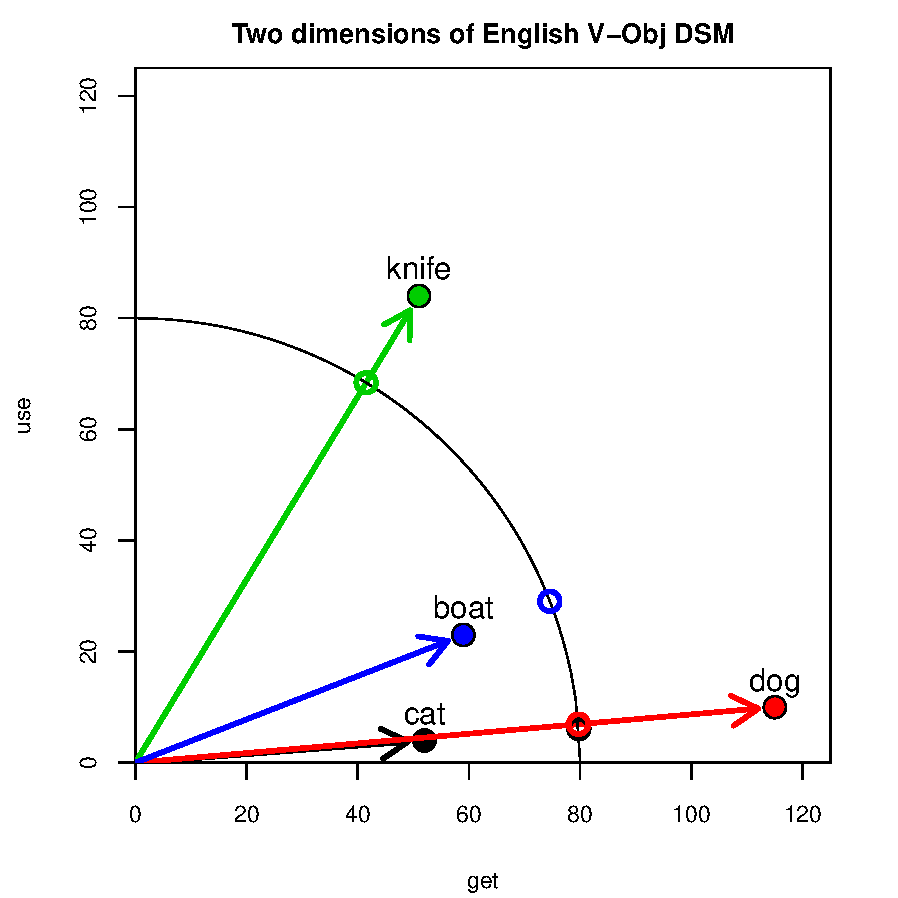
\includegraphics[width=6cm]{img/hieroglyph_2d_4}
    \end{column}
  \end{columns}
\end{frame}

\begin{frame}
  \frametitle{Scaling of column vectors}
  % \framesubtitle{}

  \begin{itemize}
  \item In statistical analysis and machine learning, features are
    usually \primary{centred} and \primary{scaled} so that
    \begin{align*}
      \text{mean} & \quad \mu = 0 \\
      \text{variance} & \quad \sigma^2 = 1
    \end{align*}
  \item In DSM research, this step is less common for columns of $\mathbf{M}$
    \begin{itemize}
    \item centring is a prerequisite for certain dimensionality
      reduction and data analysis techniques (esp.\ PCA)
    \item scaling may give too much weight to rare features
    \item co-occurrence matrix no longer sparse after centring!
    \end{itemize}
    \pause
  \item $\mathbf{M}$ cannot be row-normalised and column-scaled at the
    same time (result depends on ordering of the two steps)
  \end{itemize}
\end{frame}


\begin{frame}
  \frametitle{Geometric distance}
  %% \framesubtitle{}

  \begin{columns}[T]
    \begin{column}{60mm}
      \begin{itemize}
      \item \h{Distance} between vectors $\vu, \vv \in \setR^n$ \so
        (dis)\h{similarity}
        \begin{itemize}
        \item $\vu = (u_1, \ldots, u_n)$
        \item $\vv = (v_1, \ldots, v_n)$
        \end{itemize}
      \item<2-> \h{Euclidean} distance $\dist[2]{\vu}{\vv}$
      \item<3-> ``City block'' \h{Manhattan} distance $\dist[1]{\vu}{\vv}$
      \item<4-> Both are special cases of the \h{Minkowski} $p$-distance
        $\dist[p]{\vu}{\vv}$ (for $p\in [1, \infty]$)
      \end{itemize}
    \end{column}
    \begin{column}{45mm}
      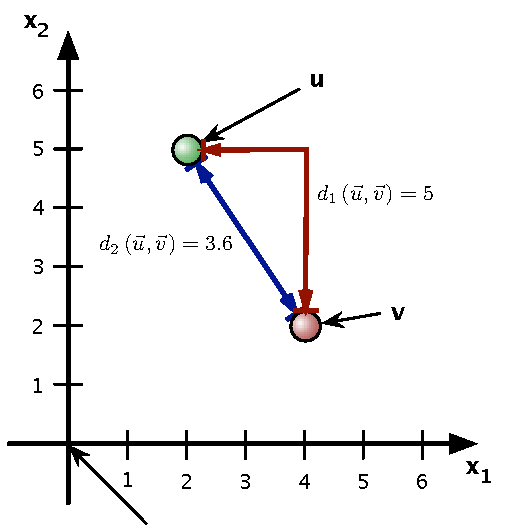
\includegraphics[width=45mm]{img/2_distance_examples}
    \end{column}
  \end{columns}
  \gap[.5]
  \only<beamer:2| handout:0>{%
    \[ \dist[2]{\vu}{\vv} \coloneq \sqrt{(u_1 - v_1)^2 + \dots + (u_n - v_n)^2} \] }
  \only<beamer:3| handout:0>{%
    \[ \dist[1]{\vu}{\vv} \coloneq \abs{u_1 - v_1} + \dots + \abs{u_n - v_n} \] }
  \only<beamer:4-| handout:1>{%
    \[ \dist[p]{\vu}{\vv} \coloneq \bigl(
    \abs{u_1 - v_1}^p + \dots + \abs{u_n - v_n}^p
    \bigr)^{1/p} \] }
  \only<beamer:5-| handout:1>{%
    \[ \dist[\infty]{\vu}{\vv} = \max \bigset{\abs{u_1 - v_1}, \ldots, \abs{u_n - v_n}} \] }
\end{frame}

\begin{frame}
  \frametitle{Geometric distance}
  %% \framesubtitle{}

  \begin{columns}[T]
    \begin{column}{60mm}
      \begin{itemize}
      \item \h{Distance} between vectors $\vu, \vv \in \setR^n$ \so
        (dis)\h{similarity}
        \begin{itemize}
        \item $\vu = (u_1, \ldots, u_n)$
        \item $\vv = (v_1, \ldots, v_n)$
        \end{itemize}
      \item \h{Euclidean} distance $\dist[2]{\vu}{\vv}$
      \item ``City block'' \h{Manhattan} distance $\dist[1]{\vu}{\vv}$
      \item Extension of $p$-distance  $\dist[p]{\vu}{\vv}$ (for $0\leq p\leq 1$)
      \end{itemize}
    \end{column}
    \begin{column}{45mm}
      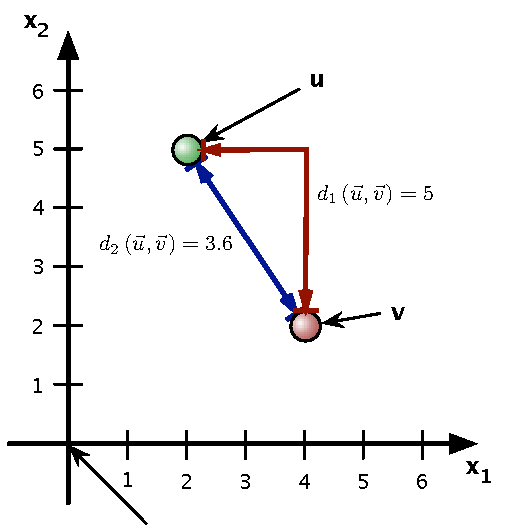
\includegraphics[width=45mm]{img/2_distance_examples}
    \end{column}
  \end{columns}
  \gap[.5]
  \[ \dist[p]{\vu}{\vv} \coloneq \abs{u_1 - v_1}^p + \dots + \abs{u_n - v_n}^p \]
  \[ \dist[0]{\vu}{\vv} = \# \bigsetdef{i}{u_i \neq v_i} \]
\end{frame}

\begin{frame}
  \frametitle{Metric: a measure of distance}
  %% \framesubtitle{}

  \begin{itemize}
  \item A \h{metric} is a general measure of the distance $\dist{\vu}{\vv}$
    between points $\vu$ and $\vv$, which satisfies the following \h{axioms}:
    \begin{itemize}
      \item $\dist{\vu}{\vv} = \dist{\vv}{\vu}$
      \item $\dist{\vu}{\vv} > 0$ for $\vu \neq \vv$
      \item $\dist{\vu}{\vu} = 0$
      \item $\dist{\vu}{\vw} \leq \dist{\vu}{\vv} + \dist{\vv}{\vw}$
        (\h{triangle inequality})
    \end{itemize}
    \pause
  \item Metrics form a very broad class of distance measures, some of which do
    not fit in well with our geometric intuitions%
    \pause
  \item E.g., metric need not be \h{translation-invariant}
    \[ \dist{\vu+\vx}{\vv+\vx} \neq \dist{\vu}{\vv} \]
    \pause\ungap
  \item Another unintuitive example is the \hh{discrete metric}
    \[
    \dist{\vu}{\vv} =
    \begin{cases}
      0 & \vu = \vv \\
      1 & \vu \neq \vv
    \end{cases}
    \]
  \end{itemize}
\end{frame}

\begin{frame}
  \frametitle{Distance vs.\ norm}
  %% \framesubtitle{}

  \begin{columns}[T]
    \begin{column}{50mm}
      \begin{itemize}
      \item<1-> Intuitively, \h{distance} $\dist{\vu}{\vv}$ should correspond to
        \h{length} $\norm{\vu-\vv}$ of displacement vector $\vu - \vv$
        \begin{itemize}
        \item $\dist{\vu}{\vv}$ is a \h{metric}
        \item $\norm{\vu-\vv}$ is a \h{norm}
        \item $\norm{\vu} = \bigdist{\vu}{\vnull}$
        \end{itemize}
      \item<2-> Such a metric is always \h{translation-invariant}%
        \gap
      \item<3-> $\dist[p]{\vu}{\vv} = \norm[p]{\vv-\vu}$
      \end{itemize}
    \end{column}
    \begin{column}{50mm}
      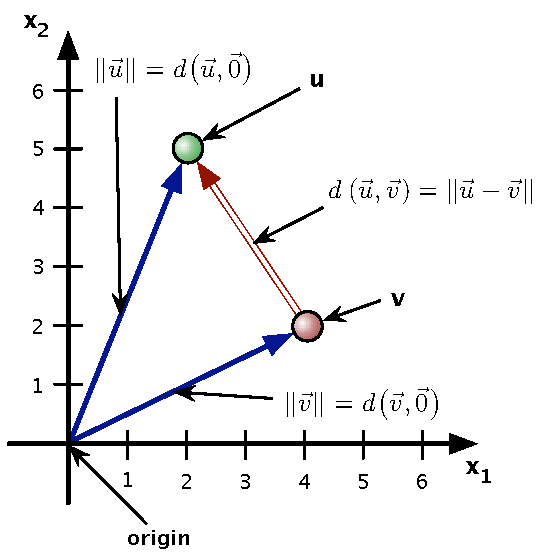
\includegraphics[width=50mm]{img/2_distance_norm}
    \end{column}
  \end{columns}

  \begin{itemize}
  \item<3-> \h{Minkowski $p$-norm} for $p\in [1,\infty]$ (not $p < 1$):
    \[
    \norm[p]{\vu} \coloneq \bigl(\abs{u_1}^p + \dots + \abs{u_n}^p\bigr)^{1/p}
    \]
  \end{itemize}
\end{frame}

\begin{frame}
  \frametitle{Norm: a measure of length}
  %% \framesubtitle{}

  \begin{itemize}
  \item A general \h{norm} $\norm{\vu}$ for the length of a vector $\vu$ must
    satisfy the following \h{axioms}:
    \begin{itemize}
    \item $\norm{\vu} > 0$ for $\vu \neq \vnull$
    \item $\norm{\lambda\vu} = \abs{\lambda}\cdot \norm{\vu}$
      (\h{homogeneity}, not req'd for metric)
    \item $\norm{\vu + \vv} \leq \norm{\vu} + \norm{\vv}$
      (\h{triangle inequality})
    \end{itemize}
    \pause\gap
  \item every norm defines a translation-invariant metric
    \[ \dist{\vu}{\vv} \coloneq \norm{\vu - \vv} \]
  \end{itemize}
\end{frame}

\begin{frame}
  \frametitle{Other distance measures}
  % \framesubtitle{}
  
  \begin{itemize}
  \item Information theory: \h{Kullback-Leibler} (KL) \h{divergence} for probability vectors (non-negative, $\norm[1]{\vx} = 1$)
    \[
    \KL{\vu}{\vv} = \sum_{i=1}^n u_i \cdot \log_2 \frac{u_i}{v_i}
    \]
    \pause
  \item Properties of KL divergence
    \begin{itemize}
    \item most appropriate in a probabilistic interpretation of $\mathbf{M}$
    \item zeroes in $\vv$ without corresponding zeroes in $\vu$ are problematic
    \item not symmetric, unlike geometric distance measures
    \item alternatives: skew divergence, Jensen-Shannon divergence
    \item[]
    \end{itemize}
    \pause
  \item A symmetric distance measure \citep{Endres:Schindelin:03}
    \[
    D_{\vu\vv} = \KL{\vu}{\vz} + \KL{\vv}{\vz} \quad \text{with} \quad \vz = \frac{\vu + \vv}{2}
    \]
  \end{itemize}
\end{frame}

\begin{frame}
  \frametitle{Similarity measures}
  % \framesubtitle{}
  
  \begin{columns}[c]
    \begin{column}{5cm}
      \begin{itemize}
        \item angle $\alpha$ between two vectors $\vu,\vv$ is given by
          \begin{align*}
            \cos \alpha &= 
            \frac{\sum_{i=1}^n u_i\cdot v_i}{
              \sqrt{\sum_i u_i^2}\cdot \sqrt{\sum_i v_i^2}}
            \\
            &= \frac{\sprod{\vu}{\vv}}{\norm[2]{\vu}\cdot \norm[2]{\vv}}
        \end{align*}
      \item<2-> \h{cosine} measure of similarity: $\cos \alpha$
        \begin{itemize}
        \item $\cos \alpha = 1$ \so collinear
        \item $\cos \alpha = 0$ \so orthogonal
        \end{itemize}
      \item<3-> distance metric: $\alpha$
      \end{itemize}
    \end{column}
    \begin{column}{6cm}
      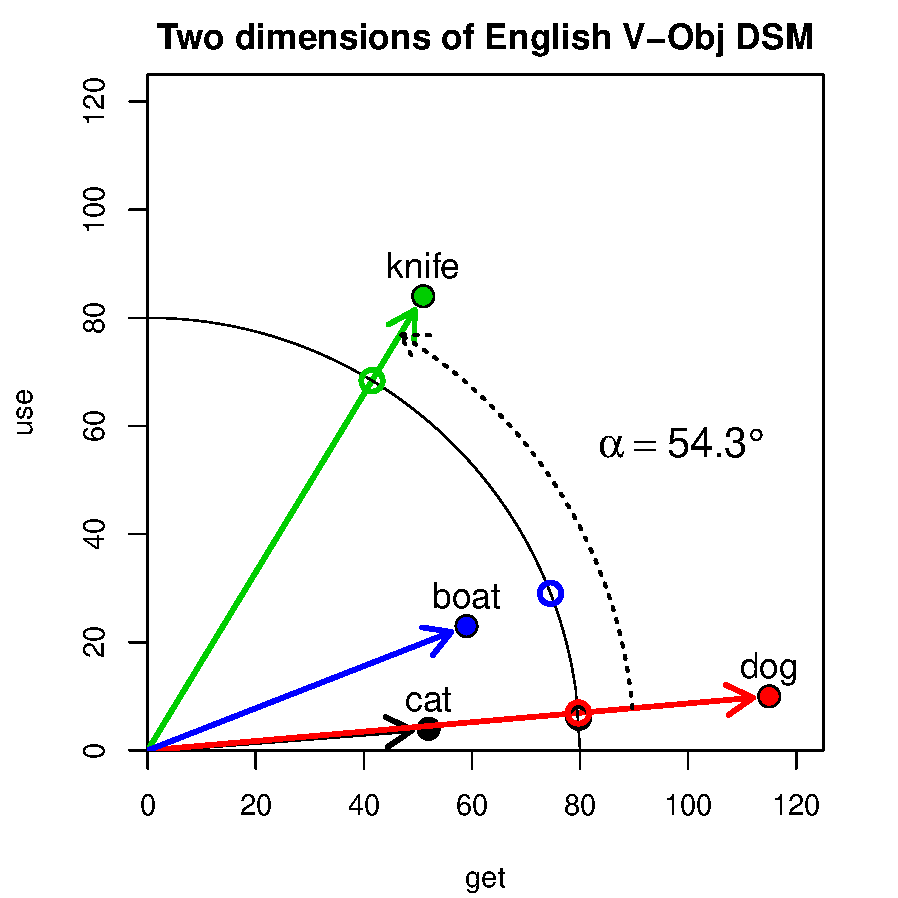
\includegraphics[width=6cm]{img/hieroglyph_2d_5}
    \end{column}
  \end{columns}
\end{frame}

\begin{frame}[fragile]
  \frametitle{Euclidean distance or cosine similarity?}

  \begin{itemize}
  \item Which is better, Euclidean distance or cosine similarity?
  \item[]
  \item<2-> They are equivalent: if vectors are normalised ($\norm[2]{\vu} = 1$),
    both lead to the same neighbour ranking
  \end{itemize}

  \onslide<3->
  \begin{align*}
    \dist[2]{\vu}{\vv} 
    &= \sqrt{\norm[2]{\vu - \vv}}
    = \sqrt{\sprod{\vu - \vv}{\vu - \vv}}
    \\
    &= \sqrt{\sprod{\vu}{\vu} + \sprod{\vv}{\vv} - 2 \sprod{\vu}{\vv}}
    \\
    &= \sqrt{\norm[2]{\vu} + \norm[2]{\vv} - 2 \sprod{\vu}{\vv}}
    \\
    &= \sqrt{2 - 2 \cos \phi}
  \end{align*}
\end{frame}

%%%%%%%%%%%%%%%%%%%%%%%%%%%%%%%%%%%%%%%%%%%%%%%%%%%%%%%%%%%%%%%%%%%%%%
\againframe<beamer:8| handout:8>{DSM_parameters}

\begin{frame}
  \frametitle{Dimensionality reduction = model compression}
  % \framesubtitle{}

  \begin{itemize}
  \item Co-occurrence matrix $\mathbf{M}$ is often unmanageably large\\
    and can be extremely sparse
    \begin{itemize}
    \item Google Web1T5: 1M $\times$ 1M matrix with one trillion
      cells, of which less than 0.05\% contain nonzero counts \citep{Evert:10a}
    \end{itemize}
  \item[\So] Compress matrix by reducing dimensionality (= rows)
    \begin{itemize}
    \item[]\pause
    \end{itemize}
  \item \h{Feature selection}: columns with high frequency \& variance
    \begin{itemize}
    \item measured by entropy, chi-squared test, \ldots
    \item may select correlated (\so uninformative) dimensions
    \item joint selection of multiple features is useful but expensive
    \end{itemize}
    \pause
  \item \h{Projection} into (linear) subspace
    \begin{itemize}
    \item principal component analysis (PCA)
    \item independent component analysis (ICA)
    \item random indexing (RI)
    \item[\hand] intuition: preserve distances between data points
    \end{itemize}
  \end{itemize}
\end{frame}

\begin{frame}
  \frametitle{Dimensionality reduction \& latent dimensions}
  %% \framesubtitle{}

  \citet{Landauer:Dumais:97} claim that LSA dimensionality reduction (and related PCA technique) uncovers \h{latent dimensions} by exploiting correlations between features.

  \begin{columns}
    \begin{column}{6.5cm}
      \begin{itemize}
      \item Example: term-term matrix
      \item V-Obj cooc's extracted from BNC
        \begin{itemize}
        \item targets = noun lemmas\\
        \item features = verb lemmas
        \end{itemize}
      \item feature scaling: association scores (modified $\log$ Dice
        coefficient)
      \item $k=111$ nouns with $f \geq 20$\\
        (must have non-zero row vectors)
      \item $n=2$ dimensions: \emph{buy} and \emph{sell}
      \end{itemize}
    \end{column}
    \begin{column}{4cm}
      \begin{center}\footnotesize
        \begin{tabular}{l|rr}
          noun & \emph{buy} & \emph{sell} \\
          \hline
          \emph{bond}      &  0.28 &  0.77\\
          \emph{cigarette} & -0.52 &  0.44\\
          \emph{dress}     &  0.51 & -1.30\\
          \emph{freehold}  & -0.01 & -0.08\\
          \emph{land}      &  1.13 &  1.54\\
          \emph{number}    & -1.05 & -1.02\\
          \emph{per}       & -0.35 & -0.16\\
          \emph{pub}       & -0.08 & -1.30\\
          \emph{share}     &  1.92 &  1.99\\
          \emph{system}    & -1.63 & -0.70
        \end{tabular}
      \end{center}
    \end{column}
  \end{columns}
\end{frame}

\begin{frame}[c]
  \frametitle{Dimensionality reduction \& latent dimensions}
  %% \framesubtitle{}
  \begin{center}
    \ungap[1]
    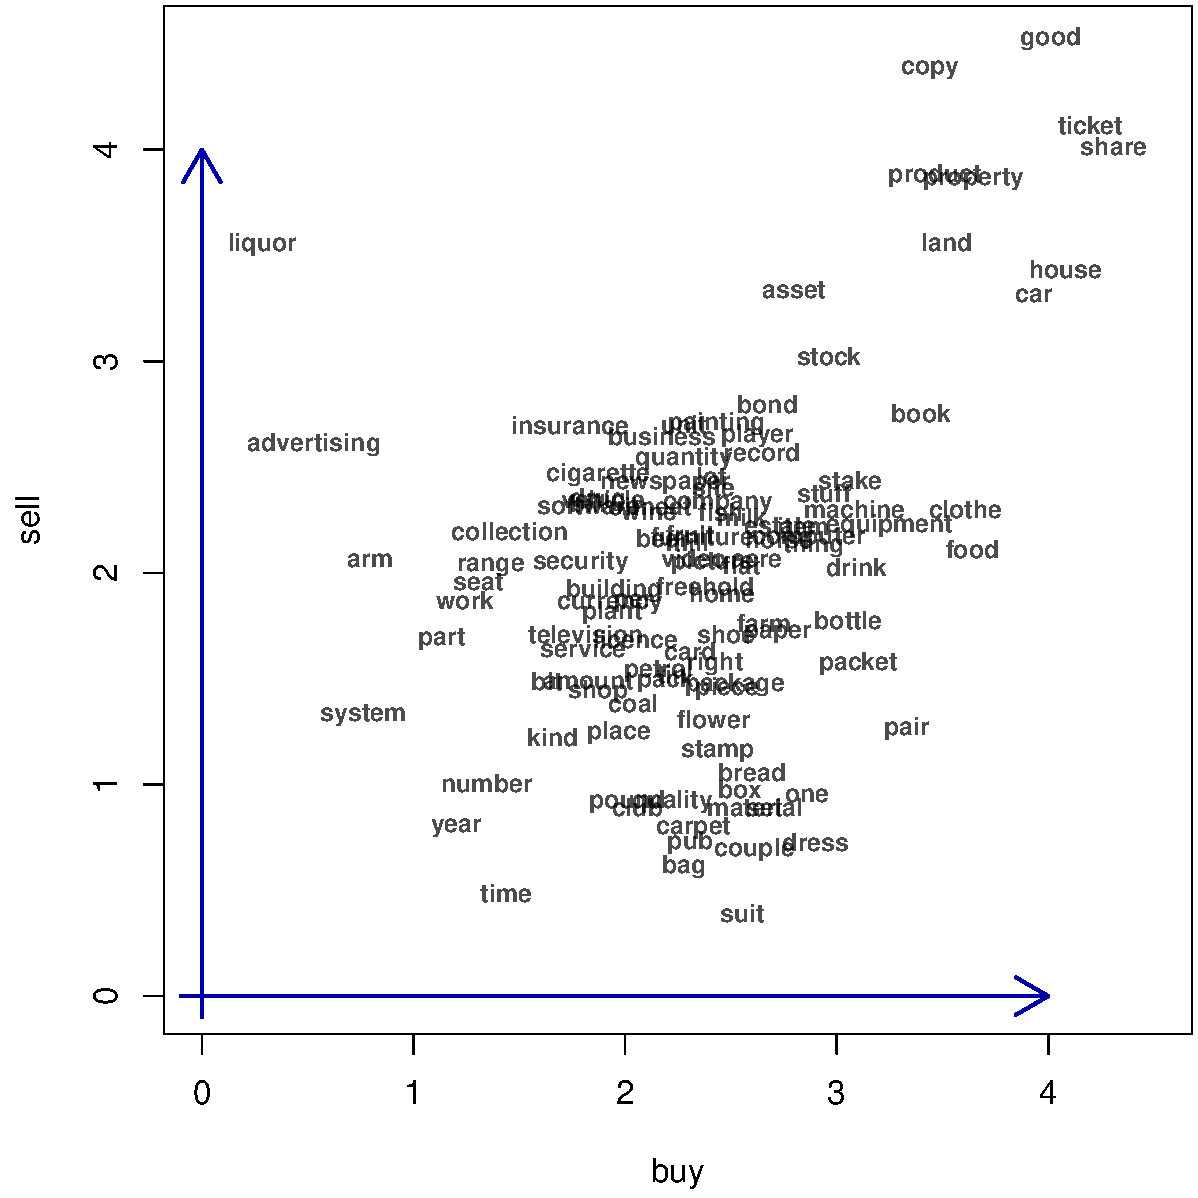
\includegraphics[width=8cm]{img/3_buy_sell_labels_only}
  \end{center}
\end{frame}

\begin{frame}
  \frametitle{Motivating latent dimensions \& subspace projection}
  %% \framesubtitle{}

  \begin{itemize}
  \item The \h{latent property} of being a commodity is ``expressed''
    through associations with several verbs: \emph{sell}, \emph{buy},
    \emph{acquire}, \ldots
  \item Consequence: these DSM dimensions will be \h{correlated}
  \item[]\pause
  \item Identify \h{latent dimension} by looking for strong correlations\\
    (or weaker correlations between large sets of features)%
  \item Projection into subspace $V$ of $k < n$ latent dimensions\\
    as a ``\h{noise reduction}'' technique \so \hh{LSA}
  \item Assumptions of this approach:
    \begin{itemize}
    \item ``latent'' distances in $V$ are semantically meaningful
    \item other ``residual'' dimensions represent chance co-occurrence
      patterns, often particular to the corpus underlying the DSM
    \end{itemize}
  \end{itemize}
\end{frame}

\begin{frame}[c]
  \frametitle{The latent ``commodity'' dimension}
  %% \framesubtitle{}
  \begin{center}
    \ungap[1]
    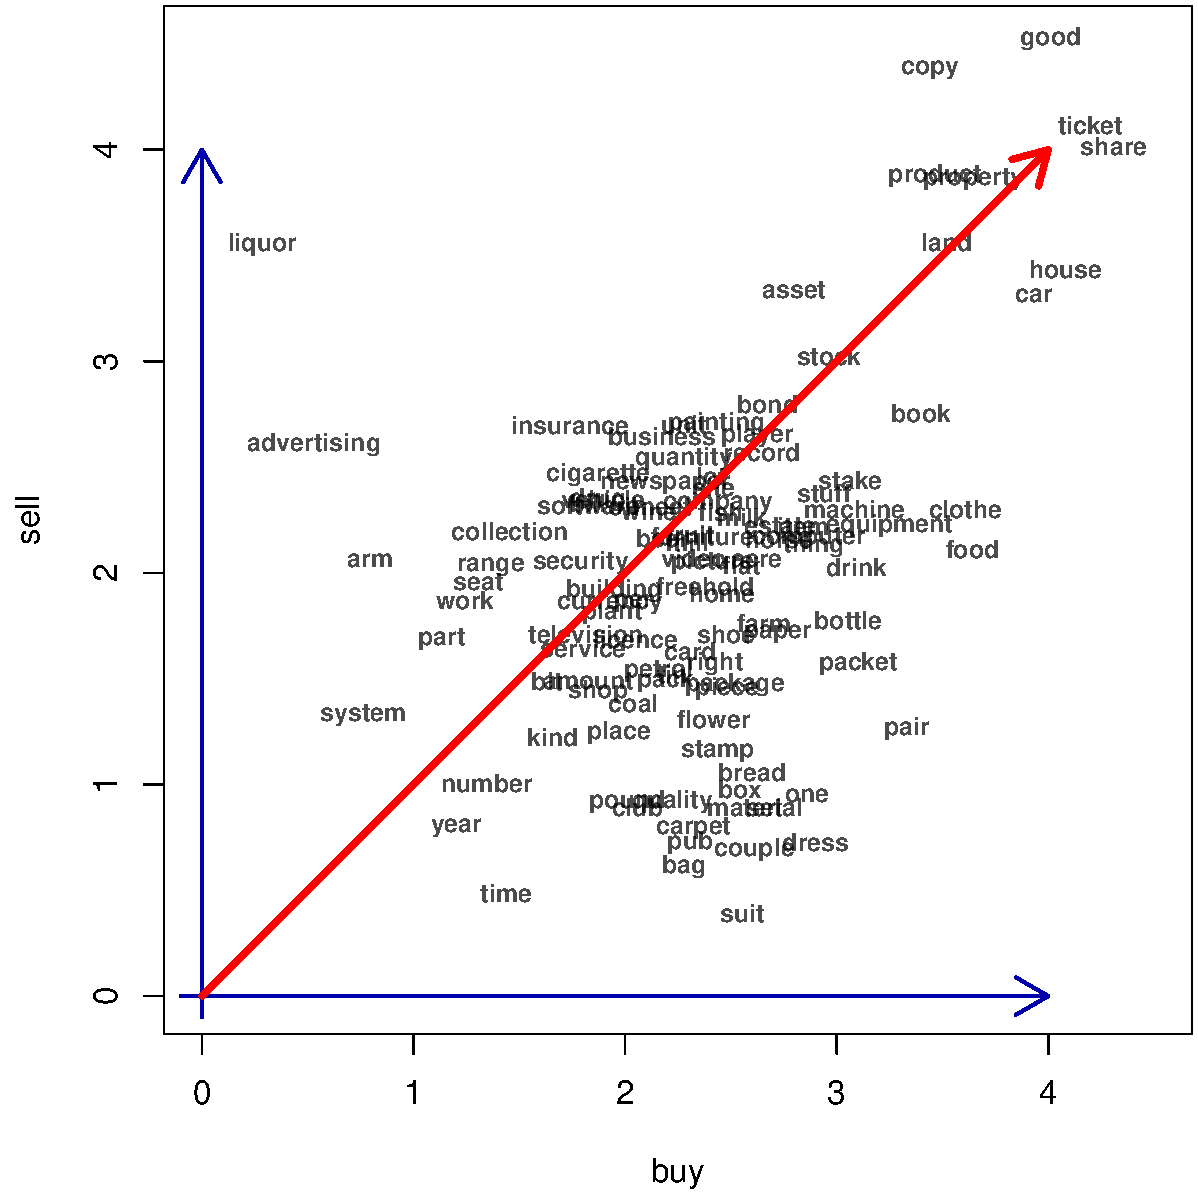
\includegraphics[width=8cm]{img/3_buy_sell_labels_latent}
  \end{center}
\end{frame}

\begin{frame}[c]
  \frametitle{Centering the data set}
  %% \framesubtitle{}

  \begin{columns}[c]
    \begin{column}{40mm}
      \begin{itemize}
      \item \h<beamer:1| handout:1>{Uncentered\\ data set}%
        \gap
      \item \h<beamer:2| handout:2>{Centered\\ data set}%
        \gap
      \item \h<beamer:3| handout:3>{Variance of\\ centered data}%
        \gap
      \end{itemize}
      \visible<beamer:3| handout:3>{%
        \[
        \sigma^2 = \tfrac{1}{k-1} \sum_{i=1}^k \norm{\vx[i]}^2
        \]
      }
    \end{column}
    \begin{column}{60mm}
      \only<beamer:1| handout:1>{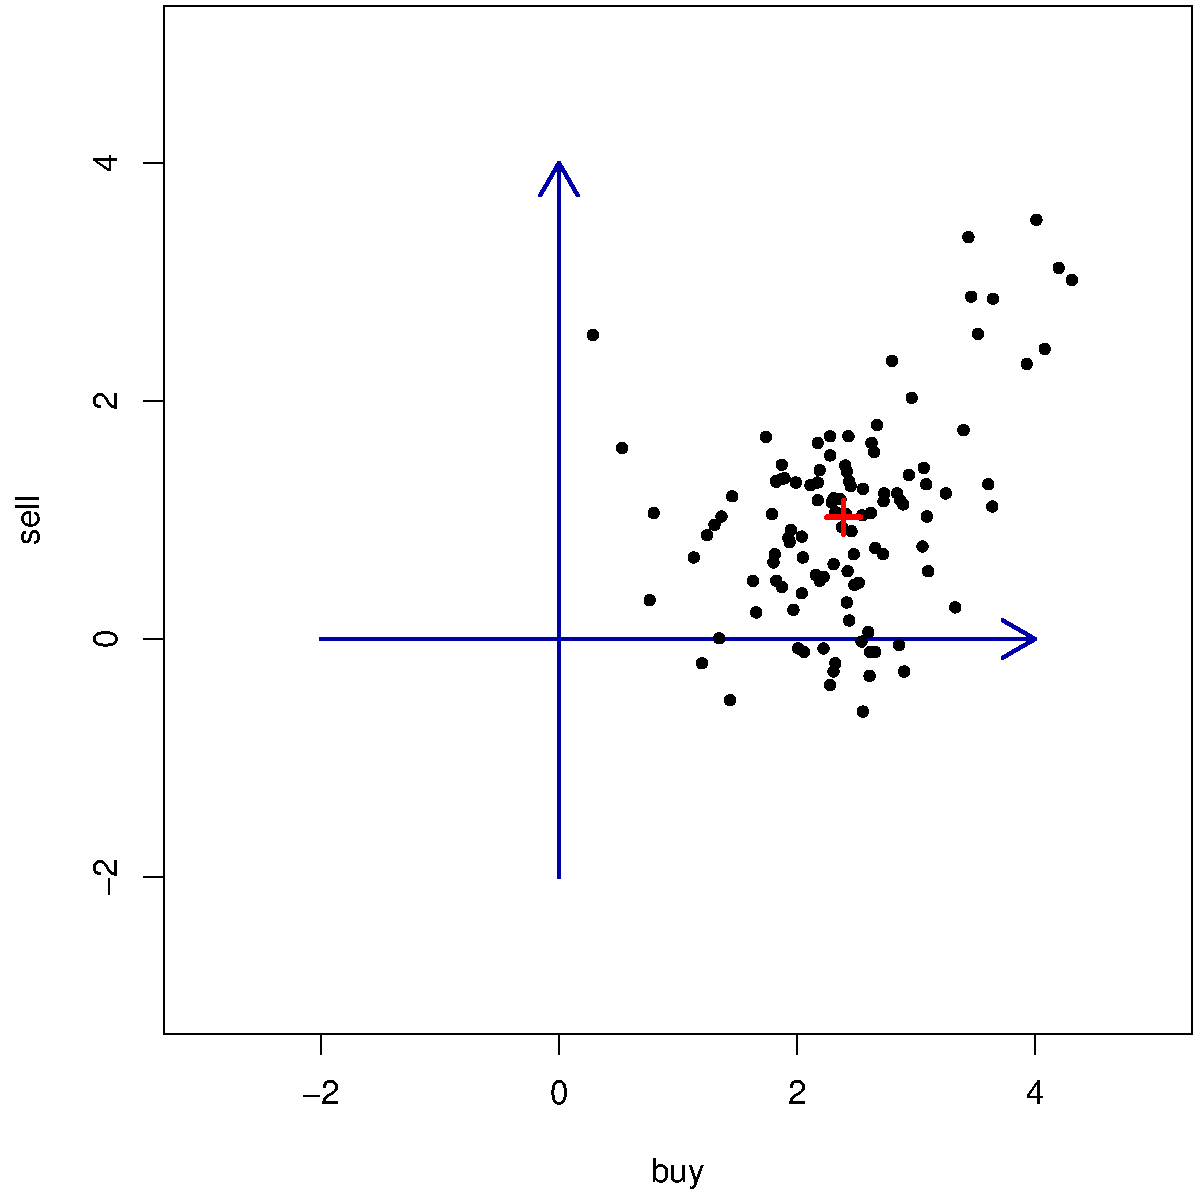
\includegraphics[width=6cm]{img/3_buy_sell_uncentered}}%
      \only<beamer:2| handout:2>{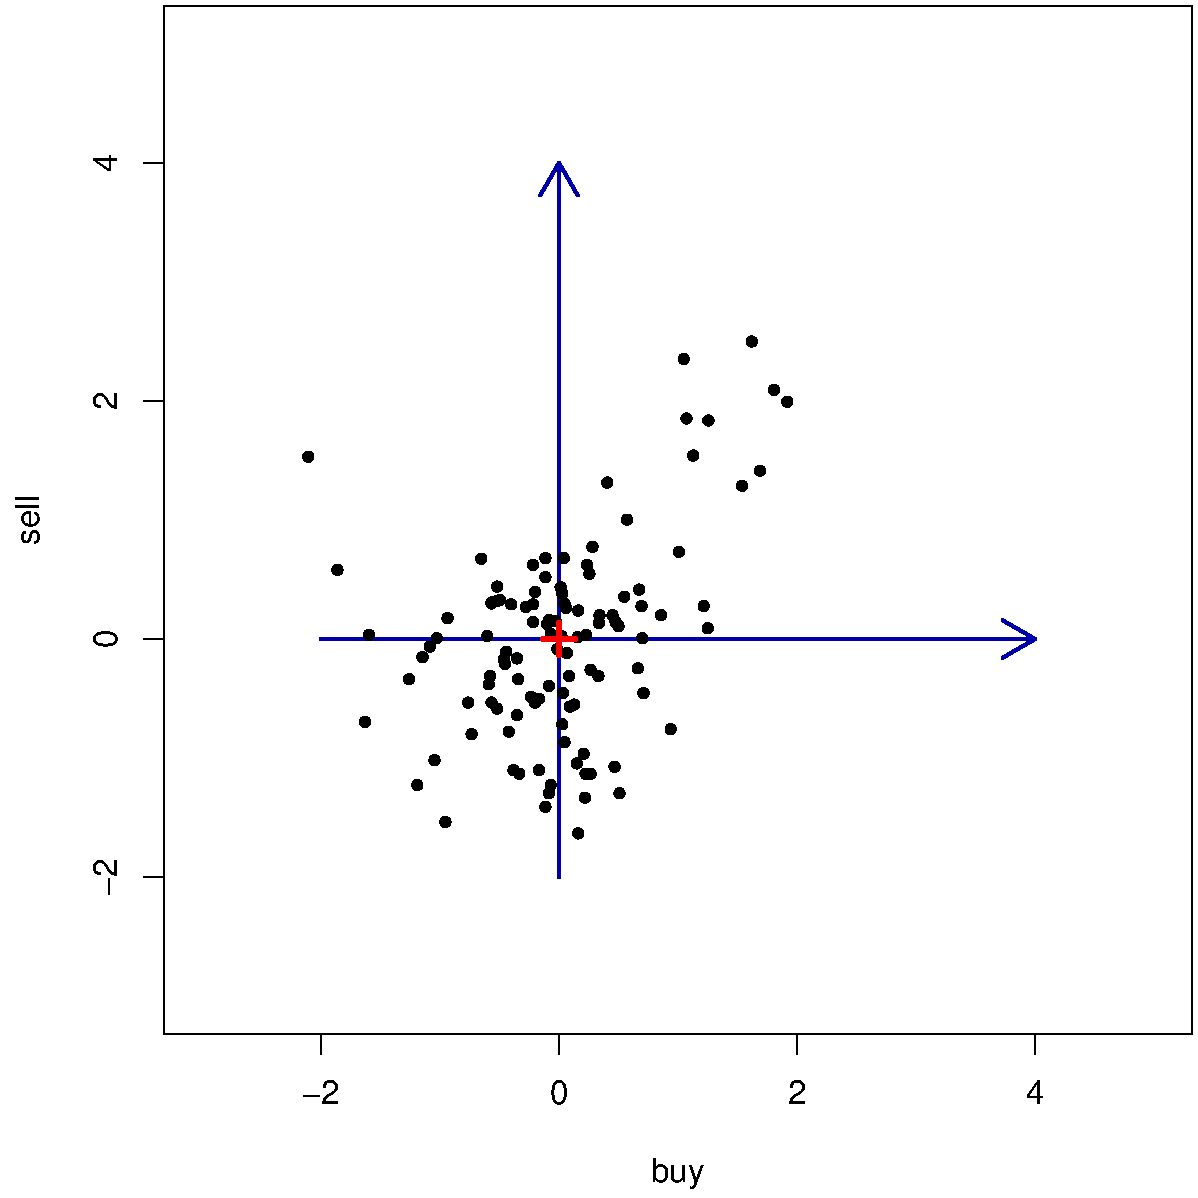
\includegraphics[width=6cm]{img/3_buy_sell_centered}}%
      \only<beamer:3| handout:3>{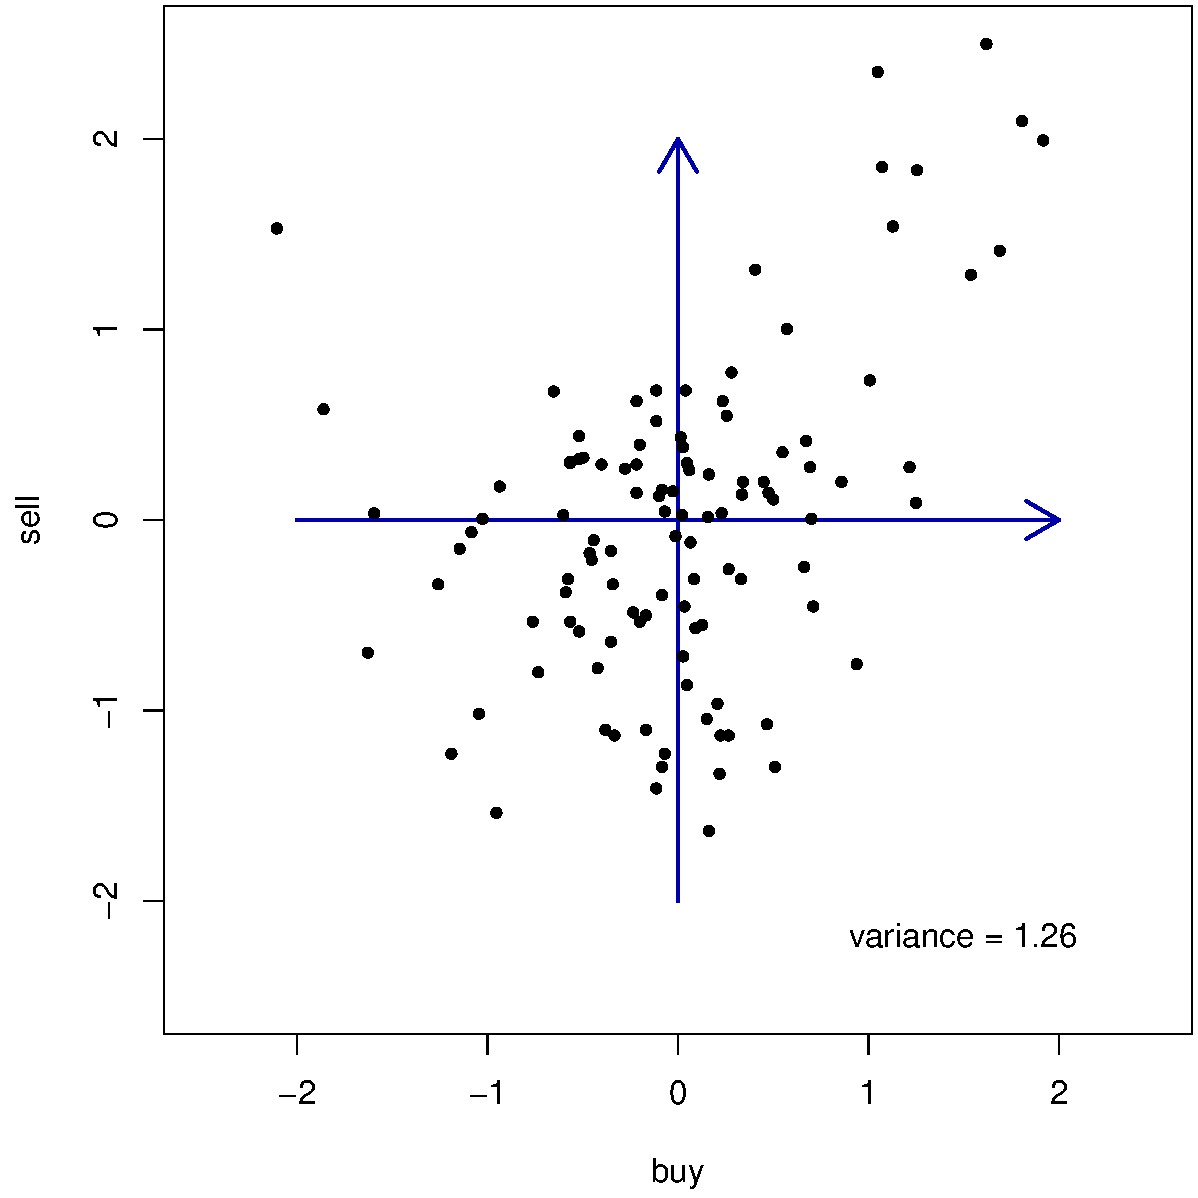
\includegraphics[width=6cm]{img/3_buy_sell_variance}}%
    \end{column}
  \end{columns}
\end{frame}

\begin{frame}<beamer:1-6| handout:1-3>[c]
  \frametitle{Projection and preserved variance: examples}
  %% \framesubtitle{}

  \begin{center}
    \only<beamer:1| handout:0>{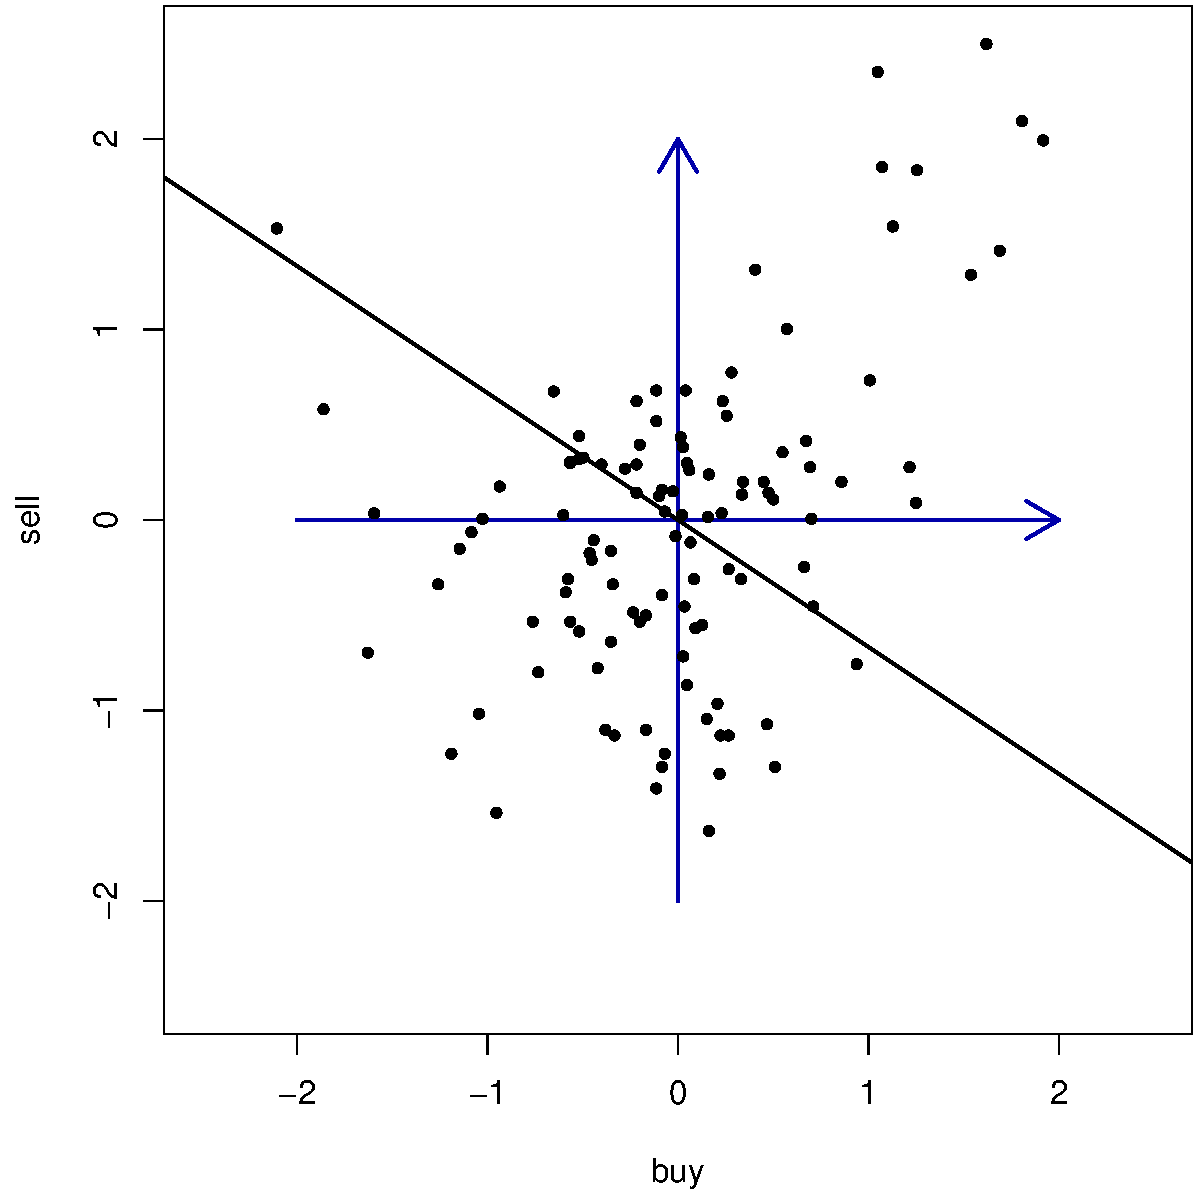
\includegraphics[width=7cm]{img/3_buy_sell_1_axis}}%
    \only<beamer:2| handout:1>{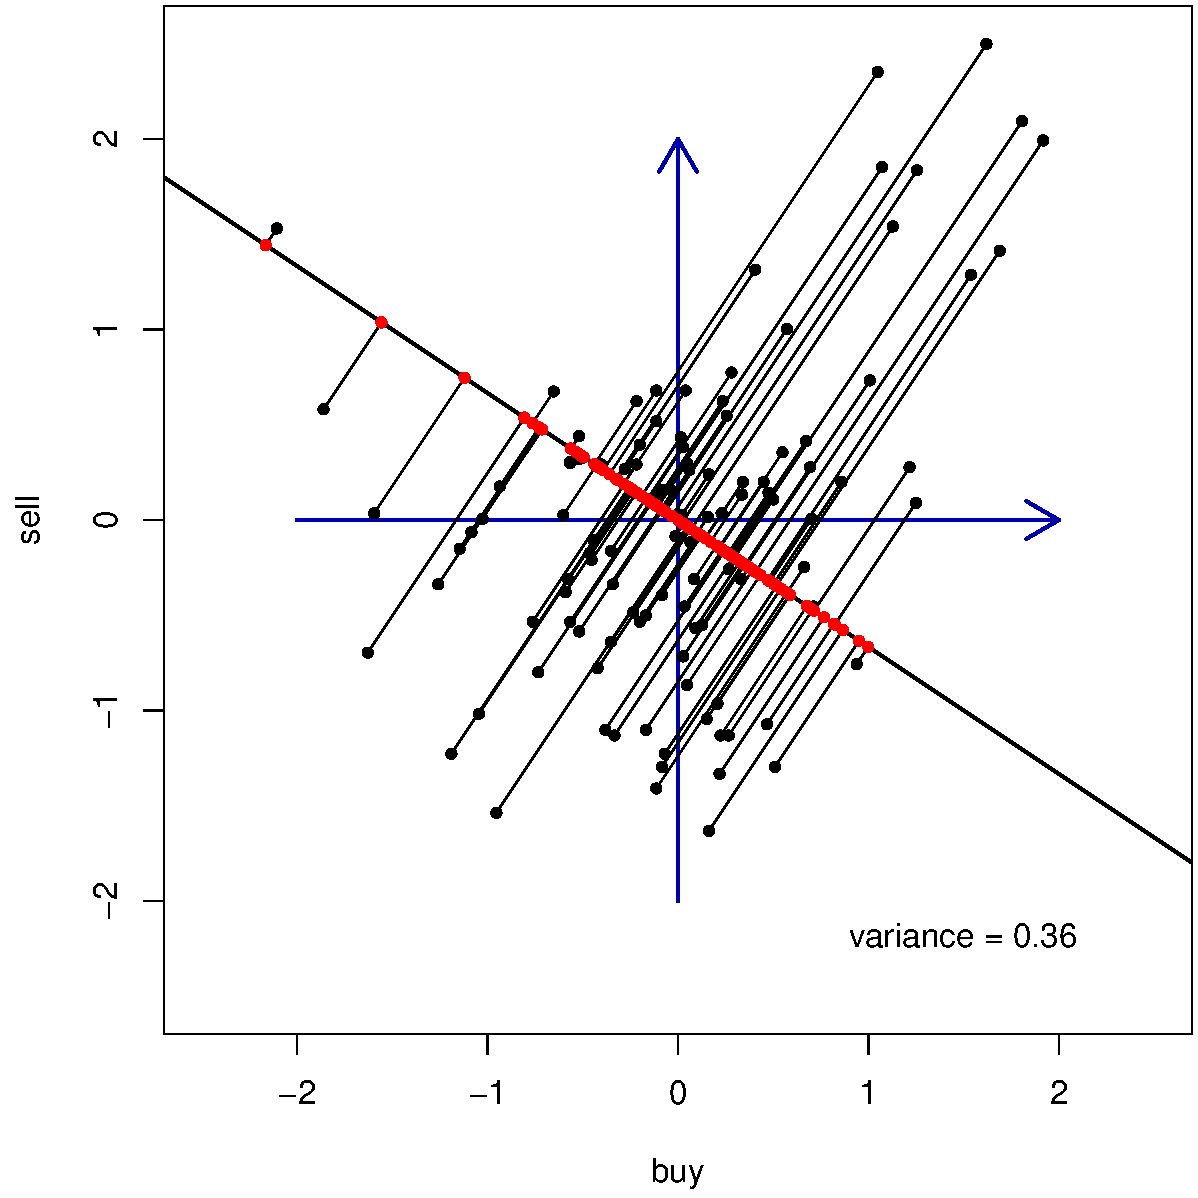
\includegraphics[width=7cm]{img/3_buy_sell_1_projection}}%
    \only<beamer:3| handout:0>{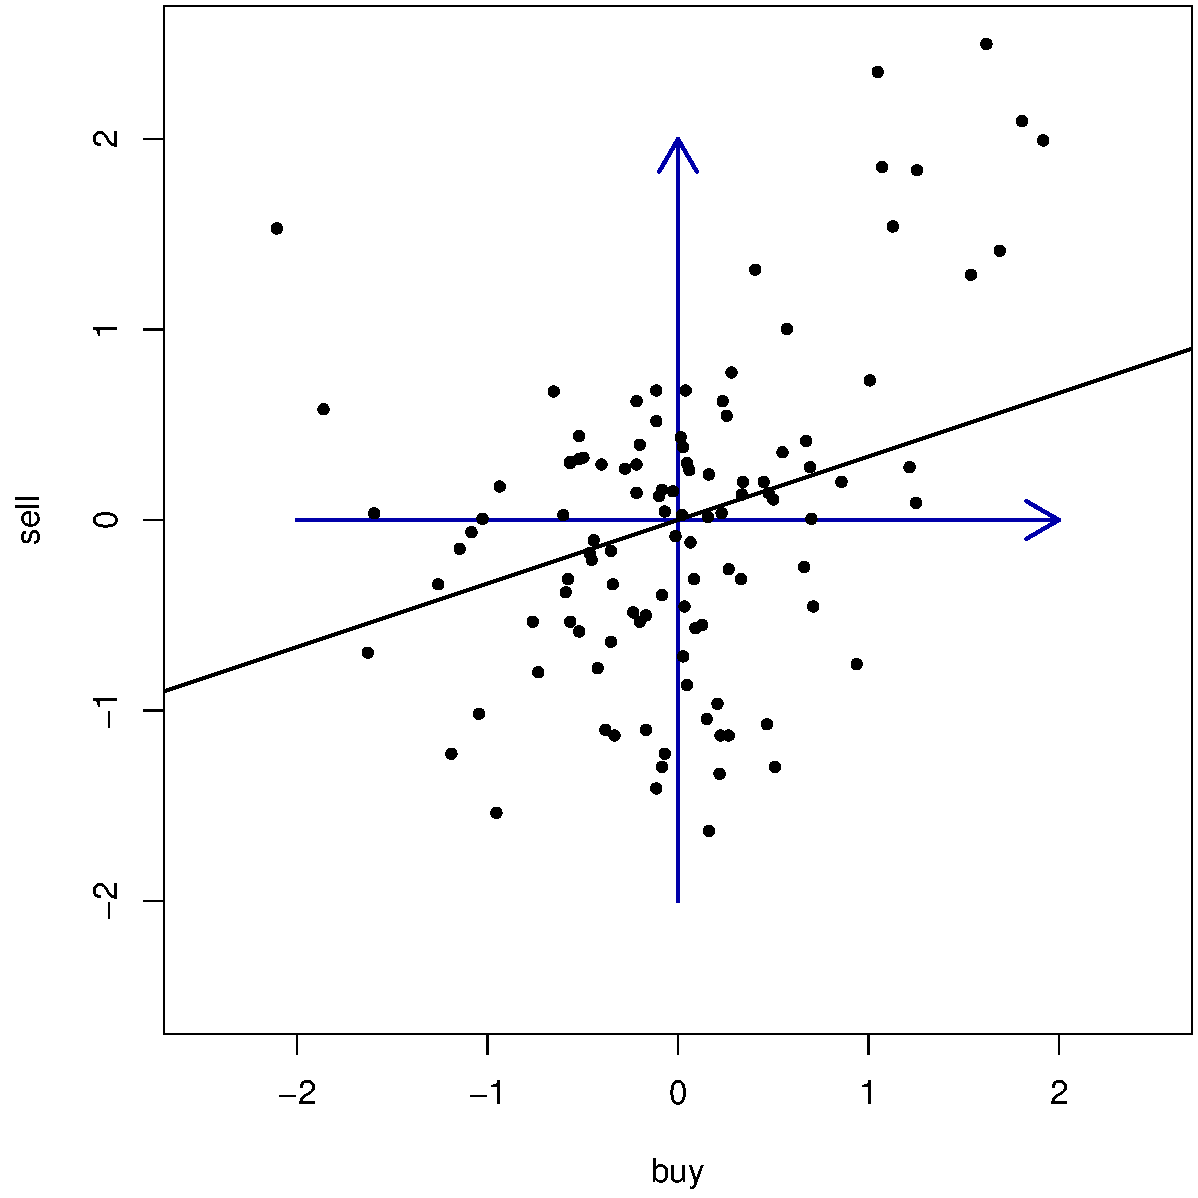
\includegraphics[width=7cm]{img/3_buy_sell_2_axis}}%
    \only<beamer:4| handout:2>{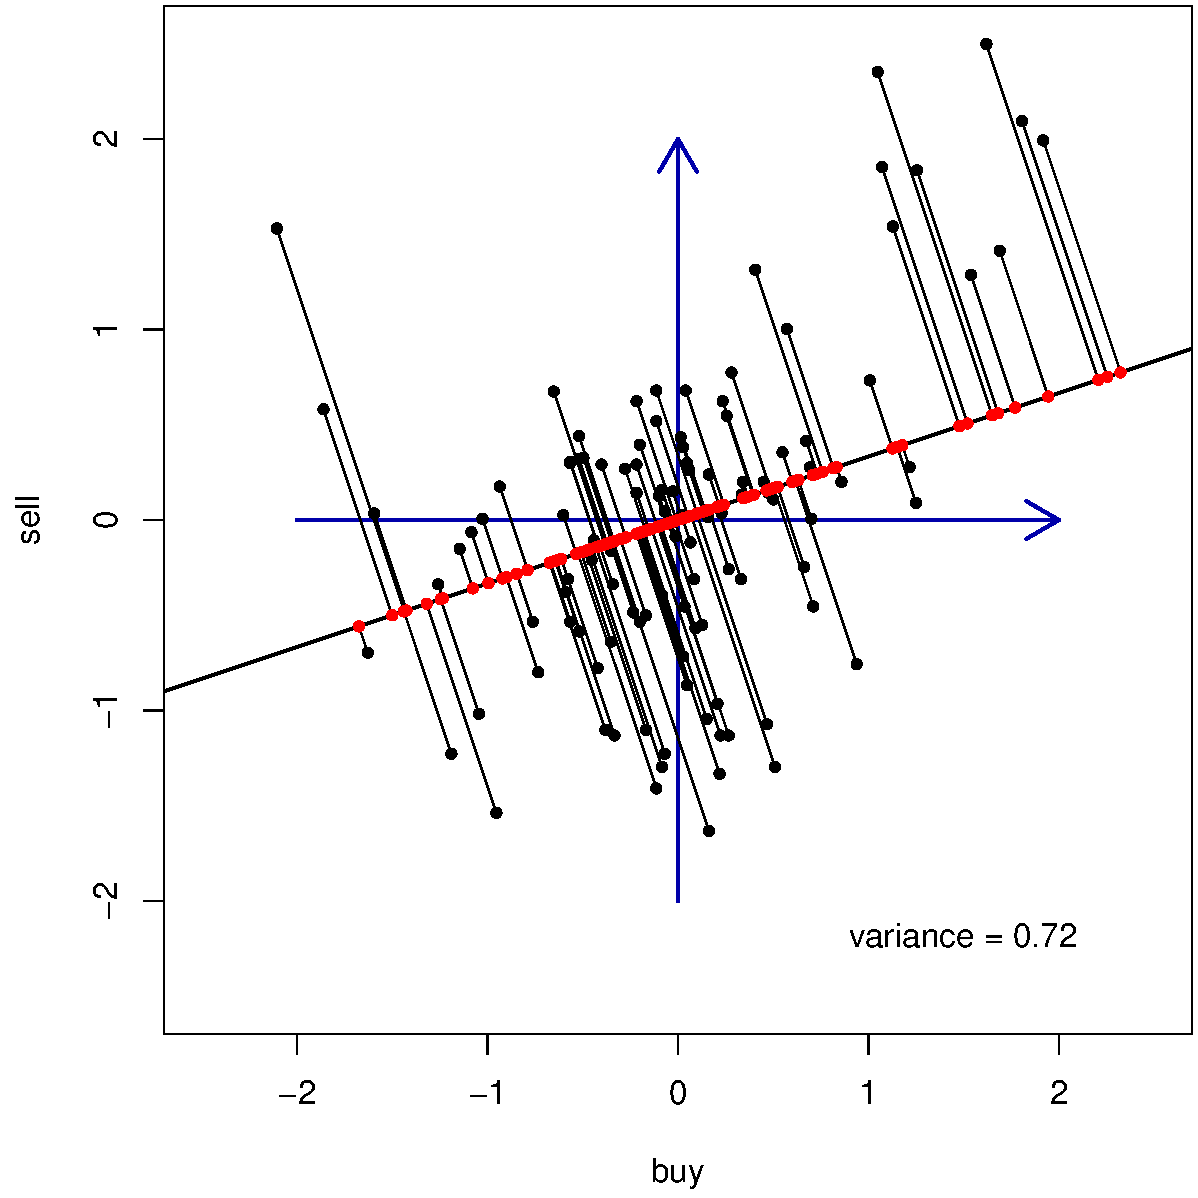
\includegraphics[width=7cm]{img/3_buy_sell_2_projection}}%
    \only<beamer:5| handout:0>{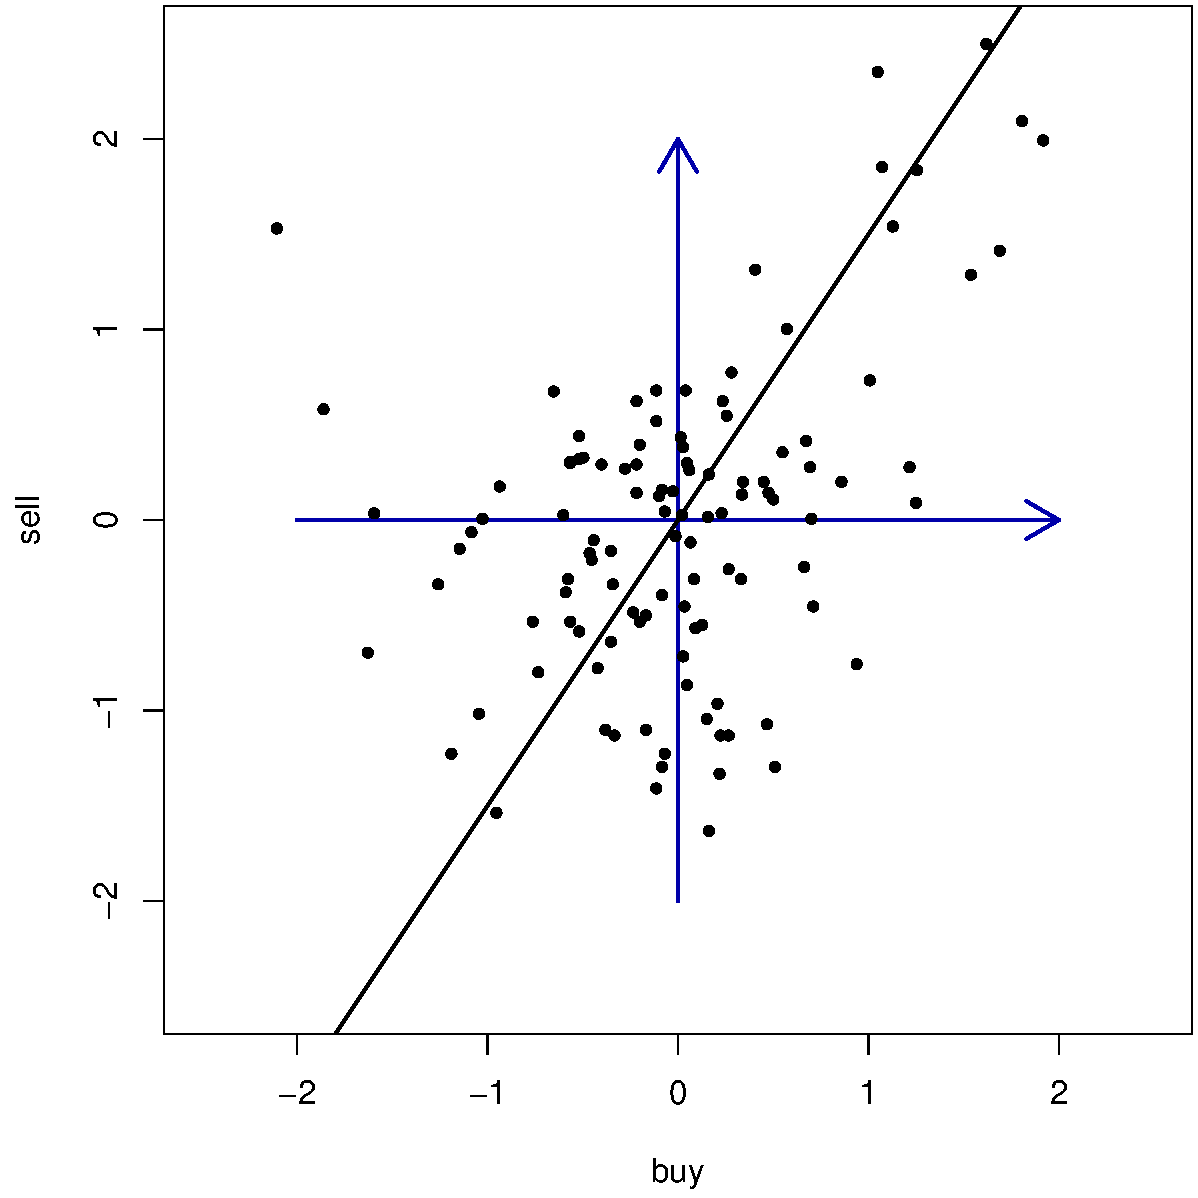
\includegraphics[width=7cm]{img/3_buy_sell_3_axis}}%
    \only<beamer:6| handout:3>{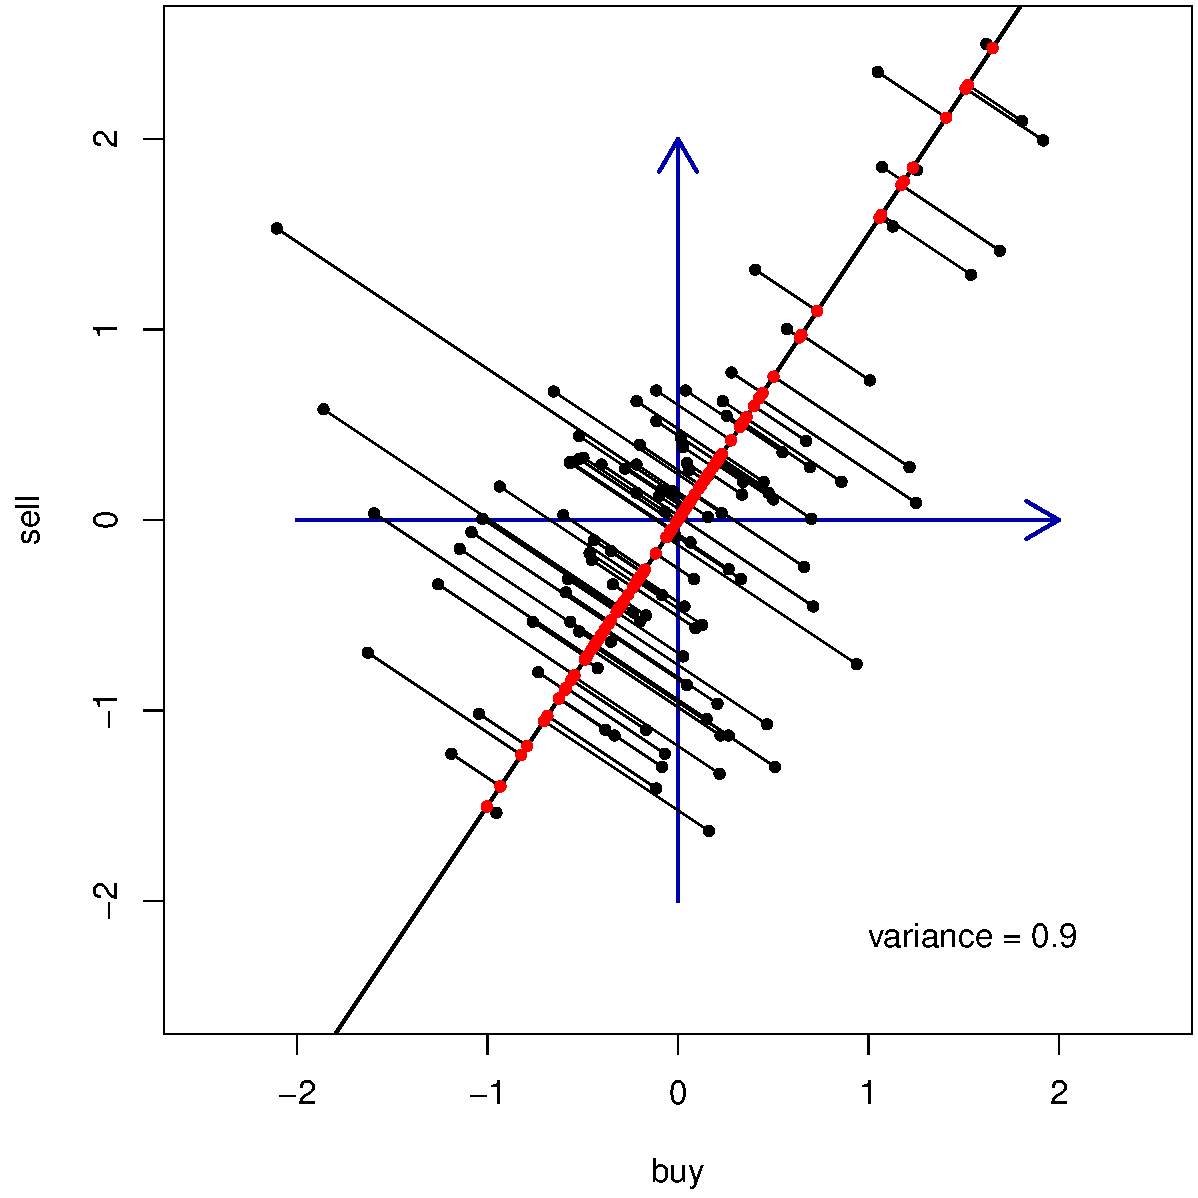
\includegraphics[width=7cm]{img/3_buy_sell_3_projection}}%
  \end{center}
\end{frame}

\begin{frame}
  \frametitle{The mathematics of projections}
  %% \framesubtitle{}

  \begin{columns}[c]
    \begin{column}{50mm}
      \begin{itemize}
      \item Line through origin given by unit vector
        $\norm{\vv} = 1$
      \item For a point $\vx$ and the corresponding unit vector $\vx' = \vx /
        \norm{\vx}$, we have \( \cos \varphi = \sprod{\vx'}{\vv} \)
      \end{itemize}
    \end{column}
    \begin{column}{50mm}
      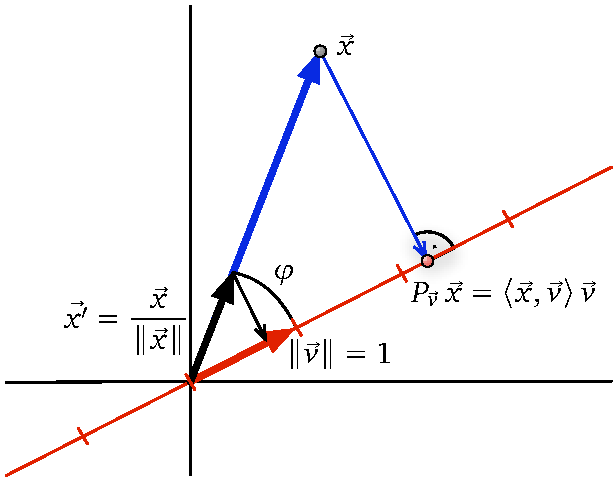
\includegraphics[width=50mm]{img/3_cosine_projection}
    \end{column}
  \end{columns}
  
  \pause
  \begin{itemize}
  \item Trigonometry: position of projected point on the line is
    $\norm{\vx}\cdot \cos\varphi = \norm{\vx}\cdot \sprod{\vx'}{\vv} =
    \sprod{\vx}{\vv}$
%  \item (projected point in original space is $\sprod{\vx}{\vv} \vv$)
  \item Preserved variance = one-dimensional variance on the line
    (note that data set is still centered after projection)
    \[
    \sigma_{\vv}^2 = \frac{1}{k-1} \sum_{i=1}^k \sprod{\vx_i}{\vv}^2
    \]
  \end{itemize}
\end{frame}

\begin{frame}[c]
  \frametitle{PCA example}
  %% \framesubtitle{}

  \ungap
  \begin{center}
    \only<beamer:1| handout:0>{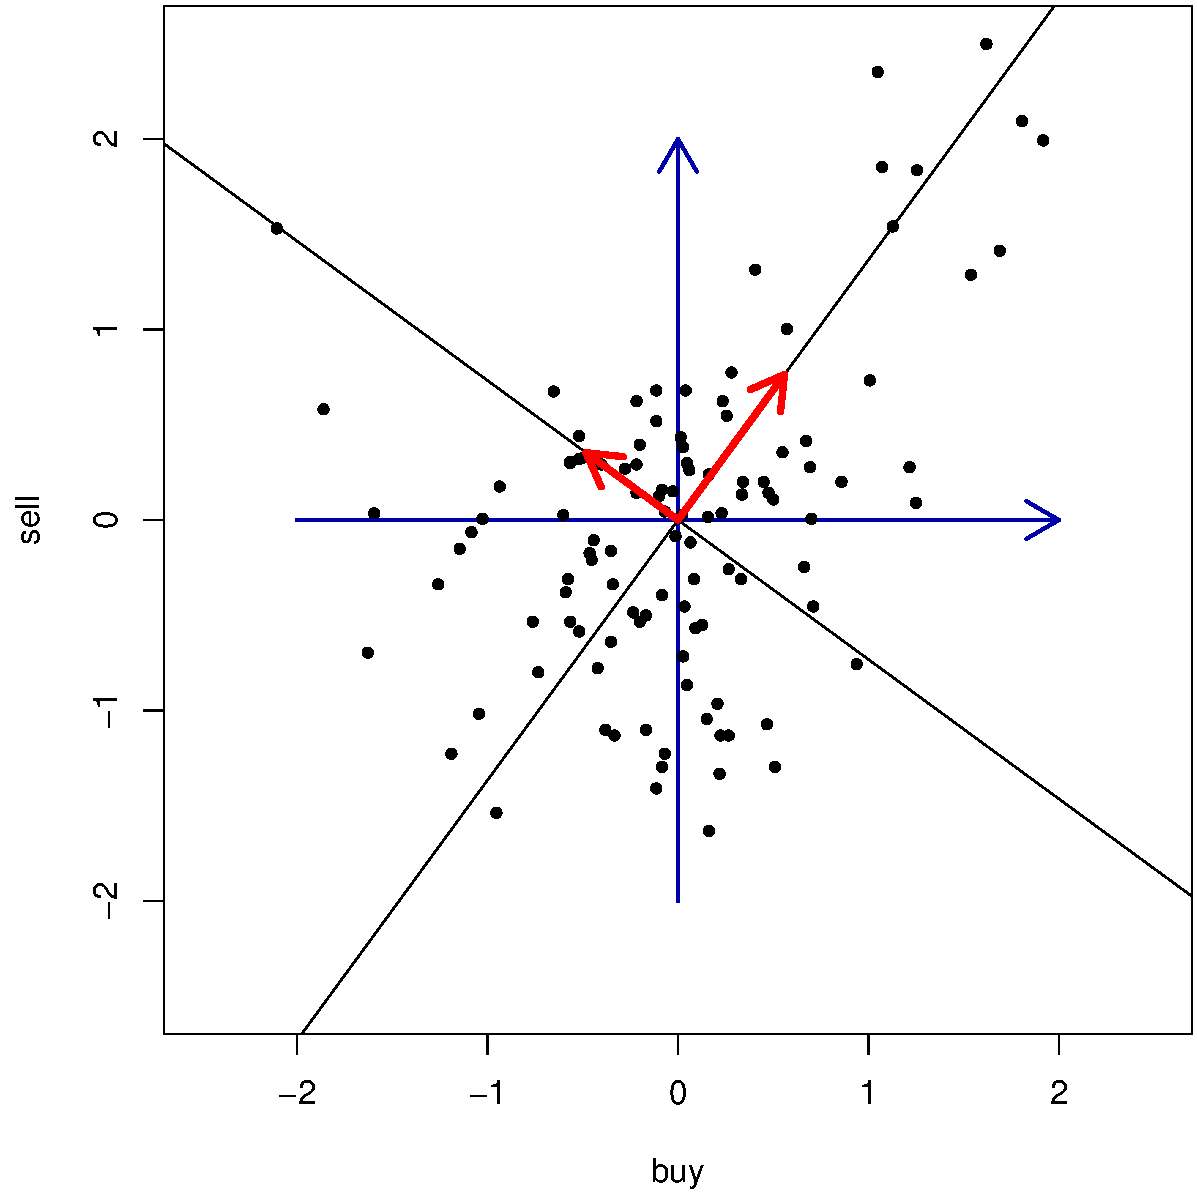
\includegraphics[width=8cm]{img/3_buy_sell_pca}}%
    \only<beamer:2| handout:1>{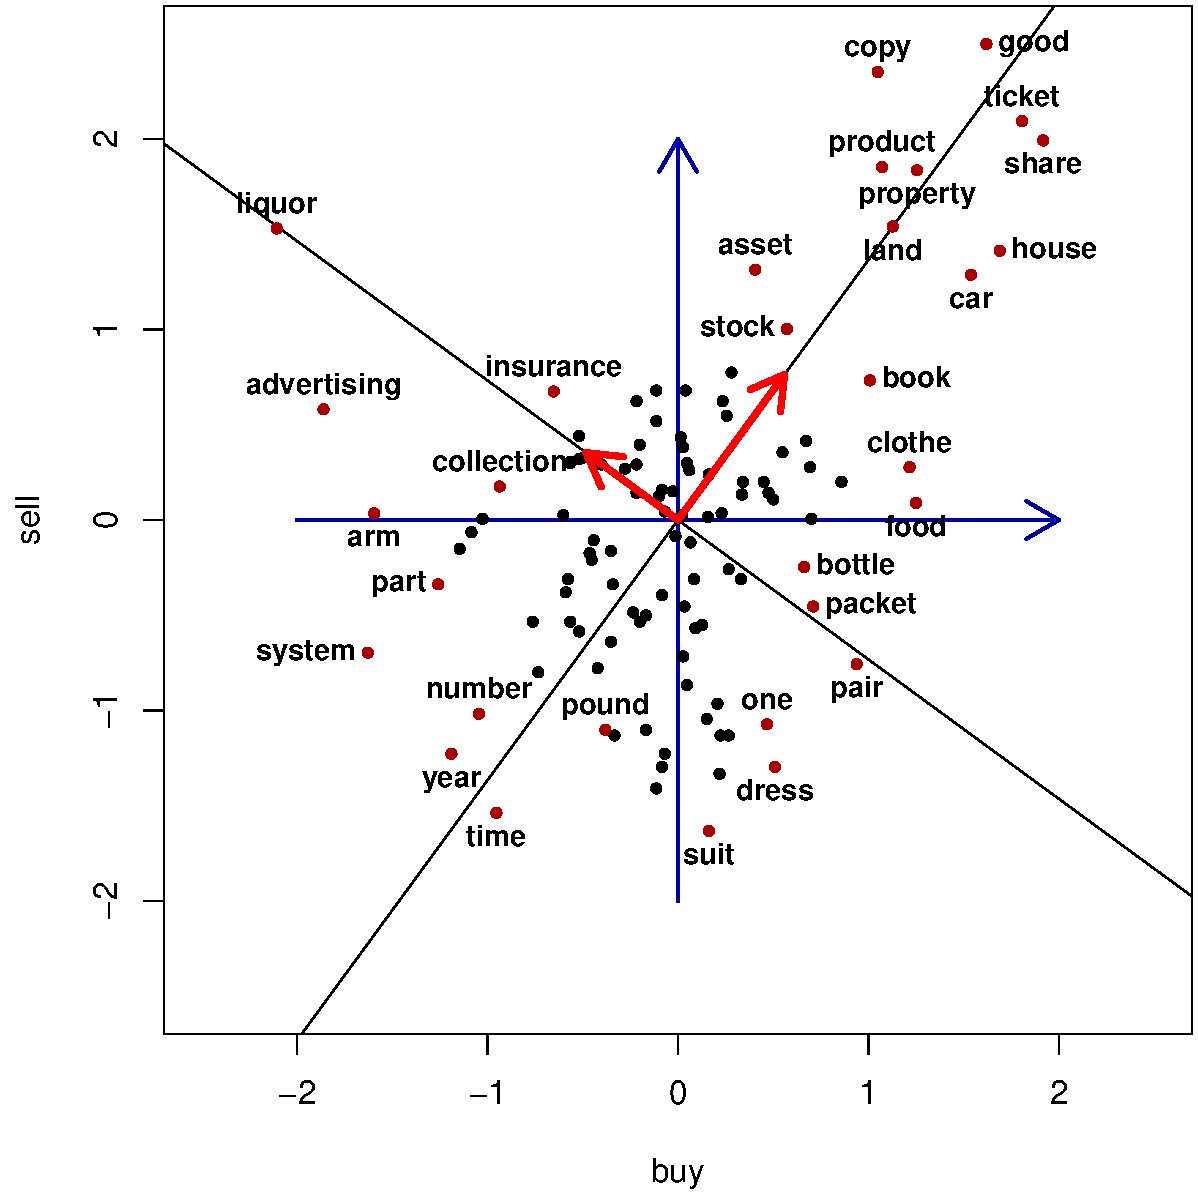
\includegraphics[width=8cm]{img/3_buy_sell_pca_labels}}%
  \end{center}
\end{frame}


%%%%%%%%%%%%%%%%%%%%%%%%%%%%%%%%%%%%%%%%%%
\subsection{Examples}

\begin{frame}
  \frametitle{Some well-known DSM examples}

  \ungap
  \begin{block} {Latent Semantic Analysis \citep{Landauer:Dumais:97}}
  \begin{itemize}
  \item term-context matrix with document context
  \item weighting: log term frequency and term entropy
  \item distance measure: cosine
  \item dimensionality reduction: SVD
  \end{itemize}
  \end{block}
 
 \begin{block} {Hyperspace Analogue to Language \citep{Lund:Burgess:96}}
  \begin{itemize}
  \item term-term matrix with surface context
  \item structured (left/right) and distance-weighted frequency counts
  \item distance measure: Minkowski metric ($1\leq p \leq 2$)
  \item dimensionality reduction: feature selection (high variance)
  \end{itemize}
  \end{block}
\end{frame}

\begin{frame}
  \frametitle{Some well-known DSM examples}

  \ungap
  \begin{block} {Infomap NLP \citep{Widdows:04}}
  \begin{itemize}
  \item term-term matrix with unstructured surface context
  \item weighting: none
  \item distance measure: cosine
  \item dimensionality reduction: SVD
  \end{itemize}
  \end{block}
 
  \begin{block} {Random Indexing \citep{Karlgren:Sahlgren:01}}
    \begin{itemize}
    \item term-term matrix with unstructured surface context
    \item weighting: various methods 
    \item distance measure: various methods
    \item dimensionality reduction: random indexing (RI)
    \end{itemize}
  \end{block}
\end{frame}

\begin{frame}
  \frametitle{Some well-known DSM examples}

  \ungap
  \begin{block}{Dependency Vectors \citep{Pado:Lapata:07}}
  \begin{itemize}
  \item term-term matrix with unstructured dependency context
  \item weighting: log-likelihood ratio
  \item distance measure: information-theoretic \citep{Lin:98a}
  \item dimensionality reduction: none
  \end{itemize}
  \end{block}
 
 \begin{block} {Distributional Memory \citep{Baroni:Lenci:10}}
  \begin{itemize}
  \item term-term matrix with structured and unstructered dependencies + knowledge patterns
  \item weighting: local-MI on type frequencies of link patterns
  \item distance measure: cosine
  \item dimensionality reduction: none
  \end{itemize}
  \end{block}
 \end{frame}

%%%%%%%%%%%%%%%%%%%%%%%%%%%%%%%%%%%%%%%%%%%%%%%%%%%%%%%%%%%%%%%%%%%%%%
\section{Building a DSM}

%%%%%%%%%%%%%%%%%%%%%%%%%%%%%%%%%%%%%%%%%%%%%%%%%%%%%%%%%%%%%%%%%%%%%%
\subsection{Scaling up}

\begin{frame}
  \frametitle{Scaling up to the real world}
  %% \framesubtitle{}

  \begin{itemize}
  \item So far, we have worked on small \hh{toy models}
    \begin{itemize}
    \item DSM matrix restricted to 2,000 -- 5,000 rows and columns
    \item small corpora (or dependency sets) can be processed within
      \textbf{R}
    \end{itemize}
    \pause
  \item Now we need to scale up to \h{real world} data sets
    \begin{itemize}
    \item for most statistical models, more data are better data!
    \item cf.\ success of Google-based NLP techniques (even if simplistic)
    \end{itemize}
    \pause
  \item Example 1: window-based DSM on BNC content words
    \begin{itemize}
    \item 83,926 lemma types with $f\geq 10$
    \item term-term matrix with 83,926 $\cdot$ 83,926 = 7 billion entries
    \item standard representation requires 56 GB of RAM (8-byte floats)%
      \pause
    \item only 22.1 million non-zero entries ($= 0.32\%$)
    \end{itemize}
    \pause
  \item Example 2: Google Web 1T 5-grams (1 trillion words)
    \begin{itemize}
    \item more than 1 million word types with $f\geq 2500$
    \item term-term matrix with 1 trillion entries requires 8 TB RAM
    \item only 400 million non-zero entries ($= 0.04\%$)
    \end{itemize}
  \end{itemize}
\end{frame}

\begin{frame}
  \frametitle{Handling large data sets: three approaches}
  %% \framesubtitle{}

  \begin{enumerate}
  \item Sparse matrix representation
    \begin{itemize}
    \item full DSM matrix does not fit into memory
    \item but much smaller number of non-zero entries can be handled
    \item[] \pause
    \end{itemize}
  \item Feature selection
    \begin{itemize}
    \item reduce DSM matrix to subset of columns (usu.\ 2,000 -- 10,000)
    \item select most frequent, salient, discriminative, \ldots\ features
    \item[] \pause
    \end{itemize}
  \item Dimensionality reduction
    \begin{itemize}
    \item also reduces number of columns, but maps vectors to subspace
    \item singular value decomposition (usu.\ ca.\ 300 dimensions)
    \item random indexing (2,000 or more dimensions)
    \item performed with external tools \so \textbf{R} can handle reduced matrix
    \end{itemize}
  \end{enumerate}
\end{frame}

\begin{frame}
  \frametitle{Sparse matrix representation}
  %% \framesubtitle{}

  \ungap
  \begin{itemize}
  \item Invented example of a \hh{sparsely populated} DSM matrix
    \begin{center}\footnotesize
      \begin{tabular}{r | cccccc}
        & eat & get & hear & kill & see & use \\
        \midrule
        boat  &   $\cdot$  & 59  &   $\cdot$  &   $\cdot$  & 39 &  23 \\
        cat   &   $\cdot$  &  $\cdot$  &   $\cdot$  &  26  & 58 &   $\cdot$ \\
        cup   &   $\cdot$  & 98  &   $\cdot$  &   $\cdot$  &  $\cdot$ &   $\cdot$ \\
        dog   &  33  &  $\cdot$  &  42  &   $\cdot$  & 83 &   $\cdot$ \\
        knife &   $\cdot$  &  $\cdot$  &   $\cdot$  &   $\cdot$  &  $\cdot$ &  84 \\
        pig   &   9  &  $\cdot$  &   $\cdot$  &  27  &  $\cdot$ &   $\cdot$ 
      \end{tabular}
    \end{center}
    \gap\pause
  \item Store only non-zero entries in compact \h{sparse matrix format}
    \begin{center}\footnotesize
      \begin{tabular}{r|r|r c r|r|r}
        row & col & value && row & col & value \\
        \cline{1-3} \cline{5-7}
        1  &  2  &  59 &&  4  &  1  &  33 \\
        1  &  5  &  39 &&  4  &  3  &  42 \\
        1  &  6  &  23 &&  4  &  5  &  83 \\
        2  &  4  &  26 &&  5  &  6  &  84 \\
        2  &  5  &  58 &&  6  &  1  &   9 \\
        3  &  2  &  98 &&  6  &  4  &  27 \\
       \end{tabular}
    \end{center}
  \end{itemize}
\end{frame}

\begin{frame}
  \frametitle{Working with sparse matrices}
  %% \framesubtitle{}

  \begin{itemize}
  \item Compressed format: each row index (or column index) stored only once,
    followed by non-zero entries in this row (or column)%
    \begin{itemize}
    \item convention: \h{column-major} matrix (data stored by columns)
    \item[]
    \end{itemize}
    \pause
  \item Specialised algorithms for sparse matrix algebra
    \begin{itemize}
    \item especially matrix multiplication, solving linear systems, etc.
    \item take care to avoid operations that create a dense matrix!
    \item[]
    \end{itemize}
    \pause
  \item \textbf{R} implementation: \texttt{Matrix} package (from CRAN)
    \begin{itemize}
    \item can build sparse matrix from (row, column, value) table
    \item unfortunately, no implementation of sparse SVD so far
    \item[]
    \end{itemize}
    \pause
  \item Other software packages: Matlab, Octave (recent versions)
  \end{itemize}
\end{frame}

%%%%%%%%%%%%%%%%%%%%%%%%%%%%%%%%%%%%%%%%%%%%%%%%%%%%%%%%%%%%%%%%%%%%%%
%% References (if any)

\frame[allowframebreaks]{
  \frametitle{References}
  \bibliographystyle{natbib-stefan}
  \begin{scriptsize}
    \bibliography{dsm}
  \end{scriptsize}
}

\end{document}
